\title{\bf{Generalised Verification for Quantified Permissions}}
\author{
	\bf{Master Thesis} \\
        	Nadja M\"uller \\
	\\
	Supervised by Alexander Summers, Prof. Dr. Peter M\"uller\\
	 Department of Computer Science \\
	ETH Zurich \\
}
\date{\today}

\documentclass[12pt]{article}
\usepackage{mathtools}
\usepackage{algorithm}
\usepackage{tabularx}
\usepackage{listings}
\usepackage{longtable}
\usepackage{silver}
\usepackage{pdfpages}
\usepackage{hyperref}

\lstset{
         numbers=left,
 }

\usepackage{color}

\definecolor{mygreen}{rgb}{0,0.6,0}
\definecolor{mygray}{rgb}{0.5,0.5,0.5}
\definecolor{mymauve}{rgb}{0.58,0,0.82}

\lstset{
  % basicstyle={\small\fontfamily{cmtt}\selectfont}
  % basicstyle={\ttfamily\selectfont\footnotesize},
  % commentstyle={\ttfamily\selectfont\footnotesize},
  breaklines=true,
  tabsize=2,
  mathescape=true,
  language=silver
  % basicstyle=\ttfamily
}

\begin{document}
\pagenumbering{gobble}
\clearpage
\newcommand*{\ident}{\hspace*{0.5cm}}
\newcommand{\wand}{\ensuremath{\mathbin{-\!\!*}}}

\begin{titlepage}

	\centering

    \vspace*{1cm}
    \Huge\textbf{Generalised Verification for Quantified Permissions}

    \vspace*{2cm}
    \Large\textbf{Master Thesis}
    
    \vspace*{1cm}
    \Large Nadja M\"uller
    
    \vspace*{0.5cm}
    Supervised by Alexander Summers,\\
    Prof. Dr. Peter M\"uller \\
    Department of Computer Science \\
    ETH Zurich
    

    \today
    
	\vfill

    \raggedright
   	
\includegraphics[width=6cm]{eth_logo_black.pdf}
    

\end{titlepage}

%\maketitle
%
\includegraphics[width=6cm]{eth_logo_black.pdf}
\newpage

\clearpage
\pagenumbering{Roman}
\tableofcontents
\newpage
\clearpage
\pagenumbering{arabic}% Arabic page numbers (and reset to 1)
\section{Abstract}
The verification infrastructure Viper supports quantified field permission of the form \(\mathbf{forall\ } x:T :: c(x) \Rightarrow acc(e(x).f, p(x))\). The quantifier may only depend on one variable and express permissions to a set of fields. Viper includes two verifiers. Carbon is based on verification condition generation, Silicon on Smallfoot-style symbolic execution. In this report, we present approaches for both types of verifiers to generalise the support for quantified permissions. We present a solution to adapt the approaches for quantified field permissions to support quantified predicate and magic wands permissions, as well as nested quantifiers. We also present rewriting rules for combining pure and permission-based quantifiers.We implemented both quantified predicate permissions and combinations of quantifiers by conjunction and implication in Carbon and Silicon.

\section{Introduction}
%viper implementation?
In order to verify heap-manipulating programs with shared mutable data structures, separation logic \cite{reynolds2002separation} and implicit frames \cite{smans2009implicit} associate an access permission with each memory location to reason about its state. 
Dynamic data structures may depend on a potentially unbounded set of memory locations. One way to define access rights to such a structure is to introduce recursive predicates defining the permissions needed. There are however access patterns which cannot be conveniently defined as a predicate, for example a random access pattern in an array.

The paper \textit{Automatic Verification of Iterated Separating Conjunctions using Symbolic Execution} \cite{isc} presented a solution to define permissions to a set of field locations regardless of the access pattern. It introduces new representation for storing the permission and symbolic values for a set of fields simultaneously, as well as symbolic rules to evaluate specific values, remove and add permissions to quantified field chunks.

The approach was implemented in the verification infrastructure Viper \cite{viper}. It includes several front-ends which translate the given programs to Viper's intermediate language. These programs can be verified with Silicon, which is based on symbolic execution, and Carbon, a verification condition generator. There are currently three features of Viper handling unbounded heap structures. Using predicates, it can handle data structures which are recursively defined, magic wands \cite{magicwand} can be used to keep track of partial data structures and quantified field permissions \cite{isc} allow us to express data structures ignorant of the way they are later accessed. 

This project presents the generalisation of the current support of quantified permissions implemented in Viper. Currently, the approach mentioned supports quantified permissions of the following structure:
\begin{equation}
	\mathbf{forall} \; x:T :: c(x) \Rightarrow \mathbf{acc}( e(x).f, p(x) ) ,
\end{equation}
where {\it f} is a field of any type, {\it c(x)} is  a Boolean expression,{\it e(x)} an injective reference-typed expression and {\it p(x)} a permission expression.

As a generalisation, we introduce new approaches adapting this solution to allow quantified permissions for predicates \cite{predicates} and magic wands \cite{magicwand} instead of fields, as well as  nested quantifiers. Further we present rewriting rules to get rid of the fixed structure of quantified field permissions, allowing expressions not defining a condition \(c(x)\) and combinations of pure and permission-based quantifiers.

\subsection{Outline}

The following section presents an overview of Viper, including the approach integrated for quantified field permissions. Section \ref{genField} shows some changes to the treatment of quantified field permissions, including the support of user-given triggers in Carbon. The adapted approach for quantified predicate permissions is introduced in Section \ref{qp}, the approach for quantified magic wand permissions in Section \ref{qmw}. The rewriting rules for combinations of quantifiers are defined in Section \ref{rewriting}. The adaption necessary to support nested quantifiers is described in Section \ref{nq}. Finally, we evaluate the performance of the implementation of quantified predicates and combinations of predicates in Section \ref{evaluation}. Additionally, the appendix holds a few examples of programs newly supported in Viper.

%to be continued

\section{Background}
\label{background}
%Permissions in general
In this chapter we give an overview of the theory needed to understand the proposed generalisation of quantified permissions. The generalisation is intended as an extension to the support for quantified fields already integrated in Viper \cite{viper}\cite{viper2014}.

Viper is a verification infrastructure for permission-based reasoning and enables the development of program verifiers based on permission logics. It is designed to facilitate the implementation of verification techniques for programs, allowing developers to focus on the encoding of higher-level language features into its intermediate verification language. It includes an intermediate verification language, two automatic back-end verifiers \textit{Carbon} and \textit{Silicon}, as well as several front-ends translating other programming languages to Viper for verification. For the generalisation we allow new quantified expressions in Viper. To support the verification of these, we adapted both Carbon and Silicon. 

\textit{Carbon}  is based on verification condition generation. It translates the given Viper program to Boogie \cite{leino2008boogie}, which proves the generated code.
In Carbon, the state is modelled by maps representing the heap and permissions held.

\textit{Silicon} is based on the SMT solver Z3 \cite{de2008z3} and Smallfoot-style Symbolic Execution \cite{berdine2005smallfoot}. The symbolic state is stored in heap chunks, holding permission and values for specific locations, and path conditions, which represent the properties obtained while evaluating or executing commands.

A Viper program consists of global declarations of fields, predicates, functions, methods, and custom domains. To represent unbounded heap structures, Viper supports the following concepts: Predicates, Magic Wands and Quantified Field Permissions.

%fields, methods, functions, predicates, custom domains.
\subsection{Permissions}
Permission logics were designed to define which locations of a heap are accessible. Viper works with fractional permissions with values between 0 and 1. Any permission greater than 0 grants read access to the corresponding field location, whereas 1 denotes full permission, which additionally allows write access to a location. 
In Viper, there are various constructs for representing permission. The one most used is the accessibility predicate acc\((e_1.f, e_2)\), denoting permission to a field location \textit{f} of the reference denoted by \(e_1\). The permission amount is expressed by \(e_2\). If the permission amount is omitted, the permission amount defaults to full permission. If an expression does not include any permission expression, it is called pure.

\subsection{Program State}
The program state of Viper includes the current permissions held, as well as the assignments to program variables. The state can be manipulated by assertions, which may only depend on locations to which permission is held. The process of verifying certain properties and updating the state during the execution of expressions can be reduced to checking, inhaling and exhaling assertions. Inhaling is equal to adding the designated permission amount if the expression represents a permission (e.g. acc\((e.f)\)), or assuming a property if the assertion is pure. Exhaling translates to removing permission or asserting the properties specified. If the permission to a location is lost, we also lose information about its value.
Carbon uses maps to describe the heap and permissions held. In Silicon, the state representation includes a set of heap chunks and path conditions.

\subsection{Types and Domains}
The built-in primitive types of Viper consist of integers (Int), Boolean expressions (Bool), references (Ref) and permissions (Perm). Additionally,  polymorphic sequences such as Seq[T] and sets Set[T] are included. Domains further allow the definition of custom domain types, which may include axioms and functions to define their properties. An example of a domain can be seen in Figure \ref{domainExample}.

\begin{figure}[h]
  \centering
\begin{lstlisting}
field val: Int

domain IArray {
  function loc(a: IArray, i: Int): Ref
  function len(a: IArray): Int

  axiom len_nonneg {
    forall a: IArray :: len(a) >= 0
  }
}
\end{lstlisting}
\caption[predicate example]
   {Example of a domain. The domain \(IArray\) represents an integer array and defines two function: \(loc\) returns the location of a specific value given an array and index, \(len\) the length of the given array. In addition to these functions, the axiom \(len\_nonneg\) defines that the length of an array has to be positive. The value of a location corresponds to \(loc(a, i).val\).}
\label{domainExample}
\end{figure}

\subsection{Fields}
Fields are globally defined and have a designated type. On declaration, the field exists for all references. In order to read a field value, a permission amount greater than 0 is necessary. When writing to a field, full permission is required.

\subsection{Methods}
Methods consist of a name, arguments (potentially including out-parameters), pre- and postconditions, as well as a method body. The preconditions must include sufficient permissions to allow all heap dereferences used in the method body. During verification, the verifiers inhale the preconditions and try to prove the postconditions after the execution of the body. If a method call is executed, the called method's precondition is exhaled. Subsequently, we gain the information defined by the postcondition by inhaling.

\subsection{Functions}
Similarly to methods, functions consist of a name, preconditions, postconditions and optionally a body. Contrary to methods, the expressions within the body are restricted and must be pure. Predicates may be used in assertions.

\subsection{Recursive Predicates}
%"Predicates can be used both to abstract over concrete assertions and to write recursive specifications of heap data structures."

Recursive Predicates \cite{parkinson2005separation} are typically used to specify linked data structures such as lists and trees. A predicate definition consists of a name,  list of formal parameters and a body. Since predicates can be recursive, as in Figure \ref{recursivePredicate}, and such a predicate could potentially be unrolled endlessly, Viper treats predicate instances as opaque. Permissions and the logical facts entailed by a predicate's body are not directly available to the verifier. We use ghost operations to obtain the logical facts from a predicate instance and vice versa.
A predicate instance may be exchanged for its body via \textit{unfold}, whereas \textit{fold} exchanges the properties of the body for an instance of the predicate. Additionally, \textit{unfolding} additionally allows the temporary unfolding of a predicate while evaluating a specified expression. An example using these ghost operations can be found in Figure \ref{predicateExample}.

%example recursive
\begin{figure}[h]
  \centering
\begin{lstlisting}
field val: Int
field next:Ref

predicate list(r:Ref)
{
    acc(r.val) && acc(r.next) && (r.next != null ==> list(r.next))
}
\end{lstlisting}
\caption[recursive predicate]
   {example of a recursive predicate definition}
\label{recursivePredicate}
\end{figure}


%example
\begin{figure}[h]
  \centering
\begin{lstlisting}
field f: Int

predicate pred(r:Ref)
{
    acc(r.f)
}

method m1(r:Ref)
requires acc(pred(r))
ensures acc(pred(r))
ensures unfolding pred(r) in r.f == 0
{

    unfold pred(r)
    r.f := 0
    fold pred(r)
}
\end{lstlisting}
\caption[predicate example]
   {Simple predicate example. By unfolding the predicate in line 14, we lose the access right to the predicate instance \textit{pred(r)} and gain the access rights to the field \textit{r.f}. This allows us to write to the field. By folding the predicate again, we regain the access rights to the predicate, which allows us no exhale the predicate in line 10. Unfolding temporarily unfolds the predicate \textit{pred(r)}, after which we obtain the permission to read the field \textit{r.f}, and also the value of that field. As a result, the assertion \textit{r.f == 0} evaluates to true.}
\label{predicateExample}
\end{figure}

\subsection{Magic Wands}
A magic wand A \(\wand\) B is a binary connective, which guarantees that if the given left-hand assertion A is satisfied in any state, then that assertion and the magic wand instance can be exchanged for the right-hand assertion B. The concept of magic wands was already mentioned in the first papers of separation logic \cite{reynolds2002separation} and can be used to keep track of partial data structures during a traversal.

A magic wand instance is created using its so-called \textit{footprint}, which is a subset of the current state that satisfies the wand's semantics. The footprint itself is not directly determined by its definition. The strategy of selecting a footprint in Viper is to include all permission required by the wands right-hand side, which we cannot prove to be provided by the wand's left-hand side \cite{magicwand}.

As for the concept of predicates, automatically reasoning about magic wands has been proven to be undecidable \cite{brochenin2008almighty}. As a consequence, Viper treats an instance of a magic wand as opaque. Exchanging the left-hand side of a magic wand with its right-hand side can be done with the ghost operation \textit{apply}. It is desugared to the following statements \cite{magicwand}:

\vbox{
\begin{longtable}{ p{0.99\textwidth} } 
 \textit{apply} \(A \wand B \longmapsto\) \\ 
\ident \textit{exhale} \(A \wand B \)\\
\ident \textit{exhale} \(A\)\\
\ident \textit{inhale} \(B\),\\
\end{longtable}
}
where \(\longmapsto\) represents a translation or rewriting step.

A second ghost operation \textit{package} \(A \wand B \) calculates a suitable footprint for the instance \(A \wand B \). The operation fails, if no such footprint can be found. Otherwise, the footprint is then exchanged for a new wand instance.

%Quantified Field Permissions
\subsection{Quantified Field Permissions}
\label{qf}

The implementation of the quantified field permissions support depends on the verifier used. We first summarise how quantified field permissions are supported in the verification generator Carbon, and then explain the approach for symbolic execution, as presented in the paper \textit{Automatic Verification of Iterated Separating Conjunctions using Symbolic Execution} \cite{isc}. 

The currently supported shape of quantified field permission expression is defined as:

\begin{equation}
\mathbf{forall\ } x:T :: c(x) \Rightarrow acc(e(x).f, p(x))
\end{equation}

The Boolean expression \(c(x)\) denotes a condition, under which a set of fields, defined by the reference-typed expression \(e(x)\) and the field \(f\), gain the permission amount expressed in the permission-typed expression \(p(x)\). An example of a quantified field permission is displayed in Figure \ref{qfExample}.

\begin{figure}[h]
  \centering
\begin{lstlisting}
field f: Int

method m(r: Ref, xs:Seq[Ref])
requires r in xs
requires forall x: Ref :: x in xs ==> acc(x.f)
{
    r.f := 4
}
\end{lstlisting}
\caption[quantified field permission example example]
   {Quantified field permission example. By inhaling the permission to the field \(f\) for all references in the set \textit{xs}, we gain the permission necessary to set a new value for the field \(r.f\).}
\label{qfExample}
\end{figure}

\subsubsection{Verification Condition Generation and Quantified Field Permissions}
\label{cgqf}
In Carbon, field permissions are represented in the map \textit{Mask}. Inhaling a field permission \(x.f\) updates the permission map for the specified location denoted by \textit{Mask}\((x, f)\) and assumes  that the reference pointing to the field is non-null. In order to support quantified field permissions, it is therefore sufficient to introduce new translations for inhaling and exhaling quantified field permissions, which update the permission map \textit{Mask} for the denoted set of fields.
Inhaling and Exhaling field permissions, as well as reading or writing to a field is done as before.

\paragraph{Inhaling a Quantified Field Permission: }
In order to model the changes to the permission map \textit{Mask} as a bulk update, we create a new map \textit{qpMask} at the beginning of the translation, which replaces \textit{Mask} after completing the inhale operation. The permission amount of the new map needs to be defined for both updated and unaffected locations. This is done by translating the quantified field permission to several Boogie quantifiers. 

Potentially, the assumption defining the values of the permission mask could be defined as \textbf{assume} \(\forall x:T :: \{?\}\ c(x) \Rightarrow qpMask[e(x), f] = Mask[e(x), f] + p(x)\), where the expression within the curly brackets represents the trigger, which allows this property for a specific value \(x'\) of type \(T\) to be available to the Boogie verifier. In Boogie, a trigger has to contain the quantifier variable and cannot only consist of a variable itself. The type of expressions allowed as a trigger is restricted as well. In order to trigger the permission update for all Mask accesses \(qpMask[r, f] \), this expression should be the trigger of the given expression, but is not a valid since  \(qpMask[r, f] \) does not contain the quantifier variable \(x\). 
In order to use this trigger, we express the same property for all references \(r\), which results in an assumption of the following form: \textbf{assume} \(\forall r:Ref :: \{qpMask[r, f]\} \dots \Rightarrow qpMask[r, f] = Mask[r, f] + p(\dots)\).

In order to translate the quantified field permission, we introduce an inverse function \(e^{-1}\), which maps a location \(r\) to the corresponding value of the original quantifier variable \(x\) of type \(T\). Using the inverse function we can check, whether a location is altered by the quantifier by evaluating the condition as \(c(e^{-1}(r))\). The gained permission is equal to \(p(e^{-1}(r))\). 
The introduction of the inverse function requires, that the expression \(e(x)\) has to be injective. When inhaling a quantified field permission, the injectivity of \(e(x)\) is assumed along with the property, that all references affected by the quantifier are non-null.

The exact translation can be seen in table \ref{qfconditionInhale}.

%carbon inhale quantified field. Frame?
\begin{longtable}{| p{1\textwidth} |}
\hline
\textbf{inhale forall } \(x:T :: c(x) \Rightarrow  acc(e(x).f, p(x)) \longmapsto\)\\
\ident Let qpMask be a new Mask\\
\ident \textbf{havoc} qpMask \\
\ident \underline{c} \(:= eval(c)\)\\
\ident \underline{e} \(:= eval(e)\)\\
\ident \underline{p} \(:= eval(p)\)\\
\\
\ident \textit{/* assert e(x) is injective */} \\
\ident \textbf{assert\ }\(\forall y_1: T, y_2:T ::\{\}\ y_1  \ne y_2 \land \underline{c}(y_1) \land \underline{c}(y_2) \Rightarrow \underline{e}(y_1) = \underline{e}(y_2)\) \\
\\
\ident \textit{/* Inverse Assumptions */} \\
\ident Let  \(e^{-1}\)  be a fresh function of type  \(T \rightarrow \) \textit{Ref} \\
\ident \textbf{assume } \( \forall x:T ::\{\underline{e}(x)\}\ \underline{c}(x)  \Rightarrow e^{-1}(\underline{e}(x)) = x \) \\
\ident \textbf{assume\ } \( \forall r:\textit{Ref} ::\{e^{-1}(r)\}\ \underline{c}(e^{-1}(r))  \Rightarrow \underline{e}(e^{-1}(r)) = r \) \\
\\
\ident \textit{/* all receiver is non-null */} \\
\ident \textbf{assume } \( \forall x:T ::\{\}\ \underline{c}(x)  \Rightarrow \underline{e}(x)) != null \) \\
\\
\ident \textit{/* define updated permission */} \\
\ident \textbf{assume\ } \(\forall r:\textit{Ref} :: \{\)Mask\((r, f)\}\ \{\)qpMask\((r, f)\}\ \{e^{-1}(r)\}\) \\
\ident  \ident \ident \ident \ident \(\underline{c}(e(r)) \Rightarrow\) qpMask\((r, f) = \)Mask\((r.f) + p(e^{-1}(r))\)\\
\\
\ident \textit{/* define independent permissions */} \\
\ident \textbf{assume\ } \(\forall r:\)\textit{Ref}\( :: \{\)Mask\((r, f)\}\ \{\)qpMask\((r, f)\}\{ e^{-1}(r)\}\)\\
\ident  \ident \ident \ident \ident \( \ \neg \underline{c}(e^{-1}(r)) \Rightarrow\) qpMask\((r, f) = \) Mask\((r, f) \)\\
\ident \textbf{assume\ } \(\forall o:\)\textit{Object}\(, f_o:\)\textit{Field}\( :: \{\)Mask\((o, f) \}\ \{\)qpMask\((o, f)\}\) \\
\ident  \ident \ident \ident \ident \((f_o != f) \Rightarrow\) qpMask\((o , f) = \) Mask\((o,f) \)\\
\ident Mask \(:=\) qpMask \\
\\ \hline
\caption[carbon quantified field inhale]
   {Translating quantified field inhale operation. The triggers are for the given forall expressions are included within curly brackets. For the expressions assuming non-null receivers and injectivity, there were no triggers defined. In our adaption of this approach, we included triggers for both assumptions. The updated translation can be seen in in Figure \ref{qfconditionInhaleExtended}.}
\label{qfconditionInhale}
\end{longtable}

\paragraph{Exhaling a Quantified Field Permission: }
Exhaling a quantified field permission \(\mathbf{forall\ } x:T :: c(x) \Rightarrow acc(e(x).f, p(x))\), includes two checks. First, we assert that the expression \(e(x)\) is injective. Then, we check that we possess the permission needed for exhaling the permission for all locations. If both checks pass, we introduce the inverse function and express the permissions of the map analogous for inhaling a quantified field permission. 
The translation is displayed in table \ref{qfconditionExhale}.

%carbon exhale quantified field
\begin{longtable}{| p{1\textwidth} |}
\hline
\textbf{exhale forall } \(x:T :: c(x) \Rightarrow  acc(e(x), p(x)) \longmapsto \) \\
\ident Let qpMask be a new Mask   \\
\ident \textbf{havoc} qpMask \\
\ident \underline{c} \(:= eval(c)\)\\
\ident \underline{e} \(:= eval(e)\)\\
\ident \underline{p} \(:= eval(p)\)\\
\\
\ident \textit{/* assert e(x) is injective */} \\
\ident \textbf{assert\ }\(\forall y_1: T, y_2:T ::\{\}\ y_1  \ne y_2 \land \underline{c}(y_1) \land \underline{c}(y_2) \Rightarrow \underline{e}(y_1) = \underline{e}(y_2)\) \\
\\
\ident \textit{/* sufficient permission */} \\
\ident \textbf{assert\ } \(\forall x:T ::\{\}\ c(x) \Rightarrow \)Mask\((e(x), f) \geq \underline{p}(x)\)\\
\\
\ident \textit{/* Inverse Assumptions */} \\
\ident Let  \(e^{-1}\)  be a fresh function of type  \(T \rightarrow \) \textit{Ref} \\
\ident \textbf{assume } \( \forall x:T ::\{\underline{e}(x)\}\ \underline{c}(x)  \Rightarrow e^{-1}(\underline{e}(x)) = x \) \\
\ident \textbf{assume\ } \( \forall r:\textit{Ref} ::\{e^{-1}(r)\}\ \underline{c}(e^{-1}(r))  \Rightarrow \underline{e}(e^{-1}(r)) = r \) \\
\\
\ident \textit{/* define updated permission */} \\
\ident \textbf{assume\ } \(\forall r:\textit{Ref} :: \{\)Mask\((r, f)\}\ \{\)qpMask\((r, f)\}\ \{e^{-1}(r)\}\) \\
\ident  \ident \ident \ident \ident \(\underline{c}(e(r)) \Rightarrow\) qpMask\((r, f) = \)Mask\((r.f) - p(e^{-1}(r))\)\\
\\
\ident \textit{/* define independent permissions */} \\
\ident \textbf{assume\ } \(\forall r:\)\textit{Ref}\( :: \{\)Mask\((r, f)\}\ \{\)qpMask\((r, f)\}\{ e^{-1}(r)\}\)\\
\ident  \ident \ident \ident \ident \( \ \neg \underline{c}(e^{-1}(r)) \Rightarrow\) qpMask\((r, f) = \) Mask\((r, f) \)\\
\ident \textbf{assume\ } \(\forall o:\)\textit{Object}\(, f_o:\)\textit{Field}\( :: \{\)Mask\((o, f) \}\ \{\)qpMask\((o, f)\}\) \\
\ident  \ident \ident \ident \ident \((f_o != f) \Rightarrow\) qpMask\((o , f) = \) Mask\((o,f) \)\\
\ident Mask \(:=\) qpMask \\
\\ \hline
\caption[carbon quantified field exhale]
   {Translating quantified field exhale operation. The missing triggers indicated by empty braces are added in the adapted translation, which is defined in Table \ref{qfconditionExhaleExtended}.}
\label{qfconditionExhale}
\end{longtable}

\subsubsection{Symbolic Execution Rules for Quantified Field Permissions}
\label{seqfp}
A solution to supporting quantified field permissions in symbolic execution is presented in  \textit{Automatic Verification of Iterated Separating Conjunctions using Symbolic Execution} \cite{isc}. The approach presented introduces a new type of heap chunk, new rules for inhaling and exhaling single and quantified field permissions, as well as for reading and writing to these field values.

%Quantified Field Chunk
\paragraph{Quantified Field Chunk:}
The permission amount and value of a unquantified field is stored in the heap as a field chunk. A field chunk \((r.f) \mapsto [v, p]\) is a defined for a symbolic reference \(r\) and a field \(f\), which is mapped to the location value \(v\) and the permission amount \(p\). The value \(v\) has the same type as the field \(f\), whereas \(p\) is a permission. 

To support quantified field chunks, a new type of chunk needed to be defined, which can hold a potentially unbounded set of references and values. A straightforward implementation of the expression \(\mathbf{forall\ } x:T :: c(x) \Rightarrow acc(e(x).f, p(x))\) would result in an heap chunk of the form  \((x, f) \mapsto [v(x), c(x) ? p(x) : 0)]\), where x is of type T. The new chunk is defined for all values of type T. The permission and value depend on x. The value \(v\) is changed to a value map storing the known values of the set. In order to evaluate the permission or value of a location \(r.f\), we would be forced to check for each chunk, whether there exists an \(x\), where \(e(x)\) evaluates to the reference \(r\).

To avoid such existential queries, the representation is adapted to the form \((r.f) \mapsto [v(r), p(r)]\), where \(r\) is of type Ref. To translate the initial permission expression to that form, we again define an inverse function, which maps a location reference to the value of the corresponding quantifier variable of Type T. The resulting quantified field chunk has the form \(r.f \mapsto [v(r), c(e^{-1}(r)) ? p(e^{-1}(r)) : 0)]\). %The domain of a quantified chunk is the set of fields r', where p(r' > 0). 

To guarantee the existence of an inverse function, it is necessary that the expression \(e(x)\) must be injective. This does not restrict the data structures that can be handled by this approach as long as correctly specified.\cite{isc}

%Inhale
\paragraph{Quantified Inhaling:}
%Given a symbolic heap, a path condition and a quantified field permission, inhaling returns an updated heap and path conditions.
Inhaling a quantified field expression generates a new quantified heap chunk. In order to do that, we first evaluate the condition, receiver expression and permission expression. As a next step we introduce the inverse function of the expression \(e(x)\), which is only partially defined for the values where the given condition \(c(x)\) applies. The inverse function is defined by adding two conditions to the path conditions. As a last step, we generate the new quantified heap chunk using the previously defined inverse function  and add it to the heap. As for inhaling a field permission, the value of the field location is initially unknown. The value map, storing the values of the references included in the quantified field chunk, is initially empty.

The symbolic execution rules are presented in Table \ref{qfInhale}.

\begin{longtable}{| p{1\textwidth} | } 
\hline
\textbf{inhale}\(\ (h_0, \pi_0,  \mathbf{forall\ } x:T :: c(x) \Rightarrow acc(e(x).f, p(x))\) \{\\
\ident Let y be a fresh symbolic constant of type\( \ T\) \\
\ident \textit{/* Symbolically evaluate source-level expressions */} \\
\ident \( \mathbf{var\ } (\pi_1, \underline{c}(y)) := eval(h_0, \pi_0, c(y)) \)\\
\ident \( \mathbf{var\ } (\pi_2,\underline{e}(y)) := eval(h_0, \pi_1 \cup \{\underline{c}(y)\}, e(y)) \)\\
\ident \( \mathbf{var\ } (\pi_3,\underline{p}(y)) := eval(h_0, \pi_2, p(y)) \)\\
\ident \( \mathbf{var\ } \pi_4 := \pi_3 \backslash \{\underline{c}(y)\} \)\\
\\
\ident \textit{/* Introduce inverse function */}\\
\ident Let  \(e^{-1}\)  be a fresh function of type  \textit{Ref}\(\Rightarrow T\) \\
\ident \(  \mathbf{var\ } \pi_5 :=  \pi_4 \cup \{\forall r: \)\textit{Ref}\(\cdot \underline{c}(e^{-1}(r))  \Rightarrow \underline{e}(e^{-1}(r)) = r \} \) \\
\ident \(  \mathbf{var\ } \pi_6 :=  \pi_5 \cup \{\forall x:T \cdot \underline{c}(x)  \Rightarrow e^{-1}(\underline{e}(x)) = x \}  \) \\
\\
\ident Let  \(v\)  be a fresh value map \\
\ident \( \mathbf{var\ } h_1 :=  h_0 \cup \{r.f \mapsto [v(r), \underline{c}(e^{-1}(r)) ? \underline{p}(e^{-1}(r)) : 0] \}  \) \\
\ident \textbf{return} \( (h_1, \pi_6) \) \\
\}\\ \hline
\caption[Inhaling a Quantified Field Permission]
   {These symbolic execution rules for inhaling a quantified field permission correspond to the rules defined in Figure 2 of the paper \textit{Automatic Verification of Iterated Separating Conjunctions using Symbolic Execution} \cite{isc}. The function \textbf{eval} is used to evaluate an expression in the given symbolic state. An evaluation may update the path variables, and yields the resulting symbolic expression. The symbolic value of the evaluated condition is added temporarily to the path condition for the evaluation of e(y) and p(y).}
\label{qfInhale}
\end{longtable}

%Exhale
\paragraph{Quantified Exhaling:}
Exhaling again starts by evaluating the condition, receiver expression and permission expression. As seen for verification condition generation, we check the injectivity of the receiver expression. Afterwards, we introduce the inverse function as before and proceed to remove the permission from the heap.

\begin{longtable}{| p{1\textwidth} | } 
\hline
\textbf{exhale}\(\ (h_0, \pi_0,  \mathbf{forall\ } x:T :: c(x) \Rightarrow acc(e(x).f, p(x))\) \{\\
\ident \textit{/* Evaluate Arguments (as above) */}\\
\ident [\dots] \\
\\
\ident \textit{/* Check injectivity of receiver expression */} \\
\ident Let \(\ y_1, y_2\ \) be a fresh symbolic constants of Type \(\ T\) \\
\ident \(\mathbf{check}\ \pi_4 \models \underline{c}(y_1) \land \underline{c}(y_2) \land \underline{e}(y_1) = \underline{e}(y_2) \Rightarrow  y_1 = y_2\) \\
\\
\ident \textit{/* Introduce inverse function (as above) */}\\
\ident [\dots] \\
\\
\ident \textit{/* Remove Permissions */}\\
\ident \( \mathbf{var\ } h_1 := \) \textit{remove} \((h_0, \pi_6, f, (\lambda r \cdot \underline{c}(e^{-1}(r))\ ?\ \underline{p}(e^{-1}(r)) : 0))  \) \\
\ident \textbf{return} \( (h_1, \pi_6) \) \\
\}\\ \hline
\caption[Exhaling a Quantified Field Permission]
   {These symbolic execution rules for exhaling a quantified field permission correspond to the rules defined in Figure 2 of the paper \textit{Automatic Verification of Iterated Separating Conjunctions using Symbolic Execution} \cite{isc}. The \textbf{check} instruction is translated to a query, which is sent to the SMT solver for verification. The function \textit{remove} is defined in Table \ref{qfRemove}.}
\label{qfExhale}
\end{longtable}

Removing the permission will raise an error, if not enough permission is held. Otherwise the function will return the updated heap. Since we create a new quantified field chunk for every inhale, the permission required may be held in multiple chunks simultaneously. When removing a certain permission amount, we first filter all quantified chunks with the required field \(f\). 
We proceed to remove permissions greedily until we removed the required permission amount. Subtracting the permission for a specific chunk is expressed by defining introducing a function \(q_{current}\). After updating the permission for all quantified field chunks of field \(f\), we check that sufficient permission was taken and return the updated heap.
The symbolic execution rules for the function \textit{remove} are displayed in Table \ref{qfRemove}.

%remove
\begin{longtable}{| p{1\textwidth} |}
\hline
\textbf{remove}\(\ (h_0, \pi_0, f, q) \) \{\\
\ident Let \(h_f \subseteq h_0\) be all chunks in given state for field \(f\) \\
\ident \textit{/* Processed chunks */} \\
\ident \( \mathbf{var \ } h'_f := \emptyset \) \\
\ident \textit{/* Permission still to take */} \\
\ident \( \mathbf{var \ } q_{needed} :=  q \)   \\
\ident \textbf{foreach} \(r.f  \mapsto [v_i(r), q_i(r)] \in h_f\) \textbf{do:} \\
\ident \ident \textit{/* Determine the permissions to take from this chunk */} \\
\ident \ident \( \mathbf{var \ } q_{current} := ( \lambda r \cdot min(q_i(r), q_{needed}(r))) \)\\
\\ 
\ident \ident \textit{/* Decrease the permissions still needed */} \\
\ident \ident \(q_{needed} := (\lambda r\cdot q_{needed}(r) - q_{current}(r)) \)\\
\\
\ident \ident \textit{/* Add an updated chunk to the processed chunks */} \\
\ident \ident \( h'_f := h'_f \cup \{r.f \mapsto [v_i(r), (q_i(r) - q_{current}(r))] \} \)\\
\\
\ident \textit{/* Check that sufficient permissions were removed */} \\
\ident \(\mathbf{check}\ \pi_0 \models \forall r \cdot q_{needed}(r) = 0 \) \\
\ident \textbf{return} \( (h_1 \backslash h_f)  \cup h'_f \) \\
\}\\ \hline
\caption[Remove a Field Permission]
   {These symbolic execution rules for removing permission of a quantified field expression correspond to the rules defined in Figure 3 of the paper \textit{Automatic Verification of Iterated Separating Conjunctions using Symbolic Execution} \cite{isc}. The argument \(f\) represents a field, \(q\) contains the permission amount needed per reference.}
\label{qfRemove}
\end{longtable}

\paragraph{Inhale Field Permission:}
In order to use the remove function defined, we need to adapt the approach for inhaling and exhaling unquantified field permissions. In Silicon, inhaling a single field permission is only adapted if the field is ever used in a quantified field permission. In that case, inhaling a field permission produces a quantified field permission as well. To express the field permission \(acc(e.f, p)\)  as its equivalent quantified chunk, we define its permission as \(p\) if  the reference is equal to the location specified by the expression \(e\). The updated inhaling rules are presented in Table \ref{sqfInhale}.

\begin{longtable}{| p{1\textwidth} | } 
\hline
\textbf{inhale}\(\ (h_0, \pi_0,  acc(e.f, p)\) \{\\
\ident \textit{/* Symbolically evaluate source-level expressions */} \\
\ident \( \mathbf{var\ } (\pi_1,\underline{e}) := eval(h_0, \pi_0, e)) \)\\
\ident \( \mathbf{var\ } (\pi_2,\underline{p}) := eval(h_0, \pi_1, p) \)\\
\\
\ident Let  \(v\)  be a fresh value map \\
\ident \( \mathbf{var\ } h_1 :=  h_0 \cup \{r.f \mapsto [v(r), \}   (r = \underline{e})\ ?\ \underline{p} : 0]\) \\
\ident \textbf{return} \( (h_1, \pi_2) \) \\
\}\\ \hline
\caption[Inhaling a single Quantified Field Permission]
   {The symbolic execution rules for inhaling a field permission, where the field is quantified at some point during the program, is adapted in order to represent all permission to a quantified field as quantified chunks.}
\label{sqfInhale}
\end{longtable}

\paragraph{Exhale Field Permission:}
Exhaling a single field permission \(acc(e.f, p)\) is handled similarly. If a field is quantified, we reuse the function remove, defining the required permission as \(p\) if the location is equal to \(e.f\) and 0 otherwise. The updated exhaling rules are presented in Table \ref{sqfExhale}.

\begin{longtable}{| p{1\textwidth} | } 
\hline
\textbf{exhale}\(\ (h_0, \pi_0,  acc(e.f, p)\) \{\\
\ident \textit{/* Evaluate Arguments (as above) */}\\
\ident [\dots] \\
\\\
\ident \textit{/* Remove Permissions */}\\
\ident \( \mathbf{var\ } h_1 := \) \textit{ remove}\((h_0, \pi_2, f, (\lambda r \cdot (r = \underline{e})\ ?\ \underline{p} : 0))  \) \\
\ident \textbf{return} \( (h_1, \pi_6) \) \\
\}\\ \hline
\caption[Exhaling a Field Permission]
   {Analogous for inhaling a field permission, the symbolic execution rules for exhaling a field permission are adapted, if the field is quantified at some point during the program.}
\label{sqfExhale}
\end{longtable}

\paragraph{Evaluation}
The value information of a quantified field chunk is stored in its value map \(v\). It represents a under-specified total function and is defined per reference. A symbolic heap may consist of multiple chunks for the same field. To provide a simple translation for field-lookups, the function summarise was introduced. Given a field \(f\), it generates a value map, containing the values for all references defined, as well as the permission expressions held per location. Summarise only works with the defined heap chunks and does not consider path conditions. The symbolic execution rules are defined in Table \ref{qfSum}.

\begin{longtable}{| p{1\textwidth} | }
\hline
\textbf{summarise}\(\ (h_0, f) \) \{\\
\ident Let \(h_f \subseteq h_0\) be all quantified chunks in the given heap for field \(f\) \\
\ident Let \(v\) be a fresh value map\\
\ident \textit{/* Value summary path conditions */} \\
\ident \textbf{var } \textit{def} \(:= \emptyset \) \\
\ident \textit{/* Permission summary */} \\
\ident \textbf{var } \textit{perm} \(:= \lambda r \cdot 0\) \\
\ident \textbf{foreach } \((r.f \mapsto [v_i(r), q_i(r)]) \in h_f \) \textbf{do:} \\
\ident \ident \(\mathit{def} := \mathit{def}  \cup \{ \forall r \cdot 0 < q_i(r)  \Rightarrow v(r) = v_i(r) \} \) \\
\ident \ident \(\mathit{perm} := \lambda r \cdot (\mathit{perm}(r) + q_i(r)) \) \\
\ident \textbf{return } \((v,\mathit{def}, \mathit{perm})\) \\
\}\\ \hline
\caption[Summarise Quantified Field Permissions]
   {These symbolic execution rules for summarising quantified field permissions correspond to Figure 5 of the paper \textit{Automatic Verification of Iterated Separating Conjunctions using Symbolic Execution} \cite{isc}. It introduces a fresh value map and walks through all quantified field chunks of field \(f\), summarising the values for the defined locations and the permission for all references.}
\label{qfSum}
\end{longtable}

If we evaluate the value of a single field location \(e.f\), we first evaluate the location and summarise all heap chunks of field \(f\). After checking we hold sufficient permission, we read the value from the generated value function. The symbolic execution rules are presented in Table \ref{qfEval}.

\begin{longtable}{| p{1\textwidth} | }
\hline
\textbf{eval}\(\ (h_0, \pi_0, e.f) \) \{\\
\ident \textbf{var } \((\pi_1, \underline{e}) :=\) \textbf{eval} (\(h_0, \pi_0, e)\) \\
\ident \textbf{var } \((v, \) \textit{def}\(,\) \textit{perm}\() :=\) \textbf{summarise} (\(h_0, f)\) \\
\ident \textbf{check } \(\pi_1 \models 0 < perm(\underline{e}) \) \\
\ident \textbf{return } \(\pi_1 \cup\) \textit{def}\(, v(\underline{e})\) \\
\}\\ 
\hline
\caption[Evaluate Field Permission]
   {These symbolic execution rules evaluating the value of a field permissions correspond to Figure 6 of the paper \textit{Automatic Verification of Iterated Separating Conjunctions using Symbolic Execution} \cite{isc}. It calls the function summarise and uses the looks up the value of the given location in the returned value map.}
\label{qfEval}
\end{longtable}

\paragraph{Field Write}
A field write \(e_1.f := e_2\) is desugared into exhaling and then inhaling the access permission of the field \(e_1.f\), followed by inhaling the equality of \(e_1.f\) and \(e_2\). Exhaling the permission of the field checks whether we possess sufficient permission to write to the field. The rules are presented in Table \ref{qfWrite}.

\begin{longtable}{| p{1\textwidth} | }
\hline
\textbf{execute}\(\ (h_0, \pi_0,e_1.f := e_2) \) \{\\
\ident \textbf{exhale } \(acc(e_1.f)\) \\
\ident \textbf{inhale } \(acc(e_1.f)\) \\
\ident \textbf{inhale } \( e_1.f == e_2\) \\
\}\\ 
\hline
\caption[Evaluate Field Permission]
   {These symbolic execution rules for desugaring a field write for a quantified field.}
\label{qfWrite}
\end{longtable}

\section{Generalising Quantified Field Permissions in Carbon}
\label{genField}
The approach presented in Section \ref{cgqf} did not include any triggers for some expressions. In such a case, triggers are generated by the underlying tools. To make the behaviour of quantified expressions more reliable and to possibly reduce unnecessary invocations, we introduced triggers for these expressions. 

The non-null assumption should be triggered for all locations. It would therefore be a possibility to reformulate the assumption as a quantifier over all references. It is however sufficient to use the same trigger as the first inverse assumption, namely \(e(x)\), since this expression will be triggered via the second inverse function when accessing a field location. An injectivity assertion, on the other hand, doesn't need to be be triggered. For that purpose, we introduce a new function \textit{triggerFun}, which takes the quantifier variable as an argument.

As another extension, we added the support for user-given triggers on quantified permissions, which were previously not supported. Most generated expressions should trigger independently of that trigger. For example, it is unnecessary to add a user-given trigger to the expression defining the permissions of the map \textit{Mask}, since the user cannot define a more general trigger than \textit{Mask}\((o , f)\)  and \(qpMask\)\((o , f) \). Other triggers are necessary to ensure the desired behaviour of quantified permissions. The most obvious example would be the trigger for the second inverse assumption, which has to be triggered for each invocation of the inverse function. Instead of replacing the previously generated triggers, we add a user-given trigger to certain expressions. A user-given trigger without alterations can only be added to expressions with the same quantifier variable type as the original quantifier. Since all other quantified assumptions are already triggered by the inverse function, there is no advantage in adding a modified trigger in these cases. We add the user-given function to the first inverse assumption as well as the non-null assumption and check for sufficient permission.

If no user-given trigger is defined, we reuse the trigger-generation function provided for pure quantifiers in order to provide additional triggers. This can be helpful in cases where \(e(x)\) does not constitute a valid trigger. Since Carbon does not support nested quantifiers, the generation of triggers was adapted to not define additional variables. The adapted triggers are displayed in Table \ref{qfconditionInhaleExtended} and \ref{qfconditionExhaleExtended}.

%carbon inhale quantified field. Frame?
\begin{longtable}{| p{1\textwidth} |}
\hline
\textbf{inhale forall } \(x:T :: c(x) \Rightarrow  acc(e(x).f, p(x)) \longmapsto\)\\
\ident Let qpMask be a new Mask\\
\ident \textbf{havoc} qpMask \\
\ident \underline{c} \(:= eval(c)\)\\
\ident \underline{e} \(:= eval(e)\)\\
\ident \underline{p} \(:= eval(p)\)\\
\\
\ident \textit{/* assert e(x) is injective */} \\
\ident \textbf{assert\ }\(\forall y_1: T, y_2:T ::\{\mathit{triggerFun}(y_1), \mathit{triggerFun}(y_2)\}\ y_1  \ne y_2 \land \) \\
\ident \ident \ident \ident \ident \(\underline{c}(y_1) \land \underline{c}(y_2) \Rightarrow \underline{e}(y_1) = \underline{e}(y_2)\) \\
\\
\ident \textit{/* Inverse Assumptions */} \\
\ident Let  \(e^{-1}\)  be a fresh function of type  \(T \rightarrow \) \textit{Ref} \\
\ident \textbf{assume } \( \forall x:T ::\{\underline{e}(x)\} \{trs\}\ \underline{c}(x)  \Rightarrow e^{-1}(\underline{e}(x)) = x \) \\
\ident \textbf{assume\ } \( \forall r:\textit{Ref} ::\{e^{-1}(r)\}\ \underline{c}(e^{-1}(r))  \Rightarrow \underline{e}(e^{-1}(r)) = r \) \\
\\
\ident \textit{/* all receiver is non-null */} \\
\ident \textbf{assume } \( \forall x:T ::\{\underline{e}(x)\} \{trs\} \underline{c}(x)  \Rightarrow \underline{e}(x)) != null \) \\
\\
\ident \textit{/* define updated permission */} \\
\ident \textbf{assume\ } \(\forall r:\textit{Ref} :: \{\)Mask\((r, f)\}\ \{\)qpMask\((r, f)\}\ \{e^{-1}(r)\}\) \\
\ident  \ident \ident \ident \ident \(\underline{c}(e(r)) \Rightarrow\) qpMask\((r, f) = \)Mask\((r.f) + p(e^{-1}(r))\)\\
\\
\ident \textit{/* define independent permissions */} \\
\ident \textbf{assume\ } \(\forall r:\)\textit{Ref}\( :: \{\)Mask\((r, f)\}\ \{\)qpMask\((r, f)\}\{ e^{-1}(r)\}\)\\
\ident  \ident \ident \ident \ident \( \ \neg \underline{c}(e^{-1}(r)) \Rightarrow\) qpMask\((r, f) = \) Mask\((r, f) \)\\
\ident \textbf{assume\ } \(\forall o:\)\textit{Object}\(, f_o:\)\textit{Field}\( :: \{\)Mask\((o, f) \}\ \{\)qpMask\((o, f)\}\) \\
\ident  \ident \ident \ident \ident \((f_o != f) \Rightarrow\) qpMask\((o , f) = \) Mask\((o,f) \)\\
\ident Mask \(:=\) qpMask \\
\hline
\caption[carbon quantified field inhale]
   {The expressions generated during a quantified inhale are adapted for the first inverse function assumption and the non-null assumption. Both expressions are triggered on the expression denoting the receiver and the user-given or automatically generated triggers. The translation is adapted from Table \ref{qfconditionInhale}.}
\label{qfconditionInhaleExtended}
\end{longtable}

%carbon exhale quantified field
\begin{longtable}{| p{1\textwidth} |}
\hline
\textbf{exhale forall } \(x:T :: c(x) \Rightarrow  acc(e(x), p(x)) \longmapsto \) \\
\ident Let qpMask be a new Mask   \\
\ident \textbf{havoc} qpMask \\
\ident \underline{c} \(:= eval(c)\)\\
\ident \underline{e} \(:= eval(e)\)\\
\ident \underline{p} \(:= eval(p)\)\\
\\
\ident \textit{/* assert e(x) is injective */} \\
\ident \textbf{assert\ }\(\forall y_1: T, y_2:T ::\{\mathit{triggerFun}(y_1), \mathit{triggerFun}(y_2)\}\ y_1  \ne y_2 \land \) \\
\ident \ident \ident \ident \ident  \(\underline{c}(y_1) \land \underline{c}(y_2) \Rightarrow \underline{e}(y_1) = \underline{e}(y_2)\) \\
\\
\ident \textit{/* sufficient permission */} \\
\ident \textbf{assert\ } \(\forall x:T ::\{\underline{e}(x)\} \{trs\}\ c(x) \Rightarrow \)Mask\((e(x), f) \geq \underline{p}(x)\)\\
\\
\ident \textit{/* Inverse Assumptions */} \\
\ident Let  \(e^{-1}\)  be a fresh function of type  \(T \rightarrow \) \textit{Ref} \\
\ident \textbf{assume } \( \forall x:T ::\{\underline{e}(x)\} \{trs\} \ \underline{c}(x)  \Rightarrow e^{-1}(\underline{e}(x)) = x \) \\
\ident \textbf{assume\ } \( \forall r:\textit{Ref} ::\{e^{-1}(r)\}\ \underline{c}(e^{-1}(r))  \Rightarrow \underline{e}(e^{-1}(r)) = r \) \\
\\
\ident \textit{/* define updated permission */} \\
\ident \textbf{assume\ } \(\forall r:\textit{Ref} :: \{\)Mask\((r, f)\}\ \{\)qpMask\((r, f)\}\ \{e^{-1}(r)\}\) \\
\ident  \ident \ident \ident \ident \(\underline{c}(e(r)) \Rightarrow\) qpMask\((r, f) = \)Mask\((r.f) - p(e^{-1}(r))\)\\
\\
\ident \textit{/* define independent permissions */} \\
\ident \textbf{assume\ } \(\forall r:\)\textit{Ref}\( :: \{\)Mask\((r, f)\}\ \{\)qpMask\((r, f)\}\{ e^{-1}(r)\}\)\\
\ident  \ident \ident \ident \ident \( \ \neg \underline{c}(e^{-1}(r)) \Rightarrow\) qpMask\((r, f) = \) Mask\((r, f) \)\\
\ident \textbf{assume\ } \(\forall o:\)\textit{Object}\(, f_o:\)\textit{Field}\( :: \{\)Mask\((o, f) \}\ \{\)qpMask\((o, f)\}\) \\
\ident  \ident \ident \ident \ident \((f_o != f) \Rightarrow\) qpMask\((o , f) = \) Mask\((o,f) \)\\
\ident Mask \(:=\) qpMask \\
\hline
\caption[carbon quantified field exhale]
   {Translating quantified field exhale operation. \(trs\) is a place-holder for the user-defined triggers or if no trigger was given, a set of auto-generated triggers. The triggers were adapted for both assertions and the first inverse assumptions. The translation is an adaption of Table \ref{qfconditionExhale}.}
\label{qfconditionExhaleExtended}
\end{longtable}

\section{Quantified Predicate Permissions}
\label{qp}
In order to generalise the form of quantified permissions, we lift the restriction on the type of the location. In this section we discuss how the presented solution for quantified field permission has to be adapted in order to support quantified predicate permissions. 
As the general form of a quantified predicate permission we consider the following adaption of the form presented for quantified field permissions: 
\begin{equation}
 \mathbf{forall} \   x:T :: c(x) \Rightarrow acc(pred(e_1 (x),…,e_n (x)), p(x)), 
\end{equation}
where \(c(x)\) is a Boolean expression, \textit{pred} a predicate name, \(\ e_i(x)\) denotes the expression conforming to the type of the ith arguments of the predicate \textit{pred}. The permission is denoted by the permission-based expression \(p(x)\). Introducing this new form allows us to express permissions to more complex structures such as a set of lists.

To explain the adaption needed for the implementation, we discuss the answers to the following questions \cite{isc}:
\begin{enumerate}
\item How to model the program state, including permissions and values?
\item How to check for a permission in a state?
\item How to add and remove permissions to and from a state?
\item How to evaluate (heap-dependent) expressions in a state?
\item When to preserve (frame) an expression's value across heap changes?
\end{enumerate}
%Example

For Verification Condition Generation, these questions are answered in the following Section \ref{vcgPredicate}. For Symbolic Execution, the first problem is handled in Section \ref{shr}, the second and third in Section \ref{qpInhaleSec} to \ref{pInhaleExhaleSec}. The fourth and fifth questions are answered  in Section \ref{qppVals} to \ref{SecFold}.

\subsection{Verification Condition Generation for Quantified Predicate Permissions}
\label{vcgPredicate}
In Carbon, the permission held for a predicate instance is stored in the map \textit{Mask}. The permissions held to a predicate location of the predicate \textit{pred} with n arguments is stored at \textit{Mask}\([null,\) \textit{pred'}\((arg_1, \dots, arg_n)]\), where \textit{pred'} represents a function returning a location, in Carbon a so-called field location, of the mask for the predicate \textit{pred} with given arguments. Similar to the approach for quantified predicate permissions, we introduce a translation for inhaling and exhaling quantified predicate permissions. There are no adaptions needed for the definition of the program state, nor do we need to change anything concerning the evaluation of  permissions. The implementation of the operations unfold, fold and unfolding does not have to be changed. 

As for both translations of inhaling and exhaling quantified field permissions, we introduce a new map, which later replaces the current map. For this map, we define the permissions relative to the previous map. For the locations included within a quantifier, the permission is increased or decreased by the designated amount. For the independent locations the permission remains unchanged. These include all field and magic wand locations, predicate instances of different predicate names, as well as predicate instances not satisfying the quantifier condition. The values of these locations are preserved, since neither inhaling nor exhaling quantified permissions change the values of the given locations.

To translate a quantified predicate permission, we generalise the solution presented for quantified fields. As for quantified field permissions, we evaluate the arguments, assert injectivity, introduce an inverse function  and define the updated permissions for the newly created map. We need, however, to redefine the definition of the inverse function and the injectivity criterion.

A predicate location is defined by a predicate name and a set of arguments. As before we wish to define the updated locations by quantifying over all predicates with predicate name \(pred\) and arbitrary arguments. Whereas for quantified field permission, we quantify over a generic receiver to define the general location of a field, a predicate depends on a set of arguments. The number of arguments and their type may differ for each predicate.

In order to translate the given permission to that location, we need to adapt the definition of the inverse function presented in Section \ref{qf}. As before, the inverse function is used to map a general location to the variable used in the original quantified permission expression. A new inverse function is defined for each expression. Since the predicate name is however independent of the quantifier variable, it is not necessary to include it as an argument of the inverse function. The adapted definition of the inverse function only depends on the arguments themselves.

As before, given the arguments of the predicate, the new inverse function returns a value of type \(T\) corresponding to the original value of the quantifier. The adapted inverse function is defined as:\\

\begin{tabularx}{1\textwidth}{ X}
\textbf{function }\(e^{-1}(a_1:A_1, \dots, a_n:A_n): T\) \\
\(\forall \ x:T :: c(x) \Rightarrow e^{-1}(e_1 (x),\dots,e_n (x))==x \) \\
\( \forall \ a_1:A_1,\dots, a_n:A_n ::  c(e^{-1}(a_1, \dots,a_n )) \Rightarrow e_i (e^{-1}(a_1,\dots, a_n )) = a_i \),\\
\end{tabularx}\\
where \(a_i\) represents the value ith argument of the predicate and \(A_i\) its type. The inverse function is, as before, is defined as a total function, but models a partial function since we only provide additional information if the condition is satisfied.

Similar to quantified field permissions, we have to restrict the allowed expressions for \(e_1(x), \dots, e_n(x)\) in order to guarantee the existence of the inverse function. The location expressed by the quantifier has to be injective. This is guaranteed if at least one argument expression differs for any two values of the quantifier variable. This property can be expressed by the following equation:\\

\begin{tabularx}{1\textwidth}{ X}
 \(\forall x_1:T, x_2: T :: c(x_1) \land c(x_2) \land (e_1(x_1) = e_1(x_2)) \land \dots \land  (e_n(x_1) = e_n(x_2)) \Rightarrow \) \\
\ident \ident \ident \ident \(x_1 = x_2\) \\
\end{tabularx}\\

The adapted translations of inhaling and exhaling quantified predicate permissions are depicted in Table \ref{qpcInhale} and Table \ref{qpcExhale}.

%carbon missing: triggers
\begin{longtable}{| p{1\textwidth} |}
\hline
\textbf{inhale}\(\ (h_0, \pi_0,  \mathbf{forall\ } x:T :: c(x) \Rightarrow  acc(pred(e_1 (x),\dots,e_n (x)), p(x)) \) \{\\
\ident \textbf{havoc} qpMask \\
\ident \underline{c} \(:= eval(c)\)\\
\ident \(\underline{e_1} := eval(e_1)\)\\
\ident \([\dots]\) \\
\ident \(\underline{e_n} := eval(e_n)\)\\
\ident \underline{p} \(:= eval(p)\)\\
\\
\ident \textit{/* Injectivity assertion */} \\
\ident \textbf{assert\ }\(\forall y_1:T, y_2:T\ \{triggerFun(y_1), triggerFun(y_2)\} : y_1  \ne y_2 \land  \)\\
\ident \ident \(\underline{c}(y_1) \land \underline{c}(y_2) \Rightarrow ((\underline{e_1}(y_1) \ne \underline{e_1}(y_2)) \lor \dots \lor  (\underline{e_n}(y_1) \ne \underline{e_n}(y_2))\) \\
\\
\ident \textit{/* Inverse assumptions */} \\
\ident Let  \(e^{-1}\)  be a fresh function of type  \(A_1, \dots, A_n \rightarrow T\) \\
\ident \textbf{assume } \( \forall x:T :: \{pred(\underline{e_1}(x), \dots, \underline{e_2}(x)\} \{trs)\}\ \underline{c}(x)  \) \\
\ident \ident \(\Rightarrow e^{-1}(\underline{e_1}(x), \dots, \underline{e_n}(x)) = x \}  \) \\
\ident \textbf{assume\ } \( \forall a_1: A_1, \dots, a_n: A_n :: \{e^{-1}(a_1, \dots, a_n)\} \ \underline{c}(e^{-1}(a_1, \dots, a_n))  \Rightarrow \) \\
\ident \ident \ident \(\underline{e_1}(e^{-1}(a_1, \dots, a_n)) = a_1 \ \& \ \dots \ \& \  \underline{e_n}(e^{-1}(a_1, \dots, a_n))= a_n \} \) \\
\\
\ident \textit{/* define updated permission */} \\
\ident \textbf{assume\ } \(\forall a_1:A_1, \dots,  a_n:A_N :: \{\)qpMask[\(null, pred(a_1, \dots, a_n)\)]\(\}\) \\
\ident \ident \(\{\)Mask[\(null, pred(a_1, \dots, a_n)\)]\(\}\{e^{-1}(a_1, \dots, a_n)\} \ c(e^{-1}(a_1, \dots, a_n)) \) \\
\ident \ident \( \Rightarrow qpMask[null, pred(a_1, \dots, a_n)] =\) \\
\ident \ident Mask[\(null, pred(a_1, \dots, a_n)\)] \( +  \ p(e^{-1}(a_1, \dots, a_n))\)\\
\\
\ident \textit{/* define independent permissions */} \\
\ident \textbf{assume\ } \(\forall a_1:A_1, \dots,  a_n:A_N :: \) \\
\ident \ident \(\{\)qpMask[\(null, pred(a_1, \dots, a_n)\)]\(\}(\{\)Mask[\(null, pred(a_1, \dots, a_n)\)]\(\} \) \\
\ident \ident \(\{e^{-1}(a_1, \dots, a_n)\}\ \neg \underline{c}(e^{-1}(a_1, \dots, a_n)) \Rightarrow \)\\ 
\ident \ident qpMask[\(null, pred(a_1, \dots, a_n)\)]\( == \)Mask[\(null, pred(a_1, \dots, a_n)\)] \\
\ident \textbf{assume\ } \(\forall o:Ref, f:Field :: \{\)qpMask[\(o, f\)]\(\} \{\)Mask[\(o, f\)]\(\}\) \\
\ident \ident \((obj \ne null \land \neg isPredicateField(f)\ \land \) \\
\ident \ident \(\mathit{predicateId}(f) != \mathit{predicateId}(pred)) \Rightarrow \) \\
\ident \ident \textit{perm}\((o.f , a_n)) = \) \textbf{old} \((\mathit{perm}(o.f)) \)\\
\ident Mask \(:=\) qpMask \\
\}\\ \hline
\caption[carbon quantified predicate inhale]
   {Translation of inhaling a quantified predicate permission. The corresponding translation for quantified field permissions is displayed in Table \ref{qfconditionInhale}. The translation differs in the definition of the general location, the inverse function and the injectivity assumption. Additionally, there is no need for a non-null assumptions for predicates. The independent locations include all instances not satisfying the condition \(c(x)\), as well as  all mask entries not pointing to a predicate instance of \(pred\). To distinguish predicates by the predicate name, we introduce the function \textit{predicateId}, which is unique for each predicate name and generated when translating a predicate declaration.}
\label{qpcInhale}
\end{longtable}

%carbon exhale quantified predicate
\begin{longtable}{| p{1\textwidth} |}
\hline
\textbf{exhale}\(\ (h_0, \pi_0,  \mathbf{forall\ } x:T :: c(x) \Rightarrow  acc(pred(e_1 (x),\dots,e_n (x)), p(x)) \) \{\\
\ident \textbf{havoc} qpMask \\
\ident \underline{c} \(:= eval(c)\)\\
\ident \(\underline{e_1} := eval(e_1)\)\\
\ident \([\dots]\) \\
\ident \(\underline{e_n} := eval(e_n)\)\\
\ident \underline{p} \(:= eval(p)\)\\
\\
\ident \textit{/* Injectivity assertion */} \\
\ident \textbf{assert\ }\(\forall y_1:T, y_2:T\ \{triggerFun(y_1), triggerFun(y_2)\} : y_1  \ne y_2 \land  \)\\
\ident \ident \(\underline{c}(y_1) \land \underline{c}(y_2) \Rightarrow ((\underline{e_1}(y_1) \ne \underline{e_1}(y_2)) \lor \dots \lor  (\underline{e_n}(y_1) \ne \underline{e_n}(y_2))\) \\
\\
\ident \textit{/* sufficient permission assertion*/} \\
\ident \textbf{assume\ } \(\forall x:T :: \ \{pred(\underline{e_1}(x), \dots, \underline{e_2}(x)\} \{trs)\}\ \underline{c}(x) \Rightarrow \) \\
\ident \ident Mask[\(null, pred(\underline{e_1}(x), \dots, \underline{e_n}(x))\)] \( \geq \underline{p}(x)\)\\
\\
\ident \textit{/* Inverse assumptions */} \\
\ident Let  \(e^{-1}\)  be a fresh function of type  \(A_1, \dots, A_n \rightarrow T\) \\
\ident \textbf{assume } \( \forall x:T :: \{pred(\underline{e_1}(x), \dots, \underline{e_2}(x)\} \{trs)\}\ \underline{c}(x)  \) \\
\ident \ident \(\Rightarrow e^{-1}(\underline{e_1}(x), \dots, \underline{e_n}(x)) = x \}  \) \\
\ident \textbf{assume\ } \( \forall a_1: A_1, \dots, a_n: A_n :: \{e^{-1}(a_1, \dots, a_n)\} \ \underline{c}(e^{-1}(a_1, \dots, a_n))  \Rightarrow \) \\
\ident \ident \ident \(\underline{e_1}(e^{-1}(a_1, \dots, a_n)) = a_1 \ \& \ \dots \ \& \  \underline{e_n}(e^{-1}(a_1, \dots, a_n))= a_n \} \) \\
\\
\ident \textit{/* define updated permission */} \\
\ident \textbf{assume\ } \(\forall a_1:A_1, \dots,  a_n:A_N :: \{\)qpMask[\(null, pred(a_1, \dots, a_n)\)]\(\}\) \\
\ident \ident \(\{\)Mask[\(null, pred(a_1, \dots, a_n)\)]\(\}\{e^{-1}(a_1, \dots, a_n)\} \ c(e^{-1}(a_1, \dots, a_n)) \) \\
\ident \ident \( \Rightarrow qpMask[null, pred(a_1, \dots, a_n)] =\) \\
\ident \ident Mask[\(null, pred(a_1, \dots, a_n)\)] \( -  \ p(e^{-1}(a_1, \dots, a_n))\)\\
\\
\ident \textit{/* define independent permissions */} \\
\ident \textbf{assume\ } \(\forall a_1:A_1, \dots,  a_n:A_N :: \) \\
\ident \ident \(\{\)qpMask[\(null, pred(a_1, \dots, a_n)\)]\(\}(\{\)Mask[\(null, pred(a_1, \dots, a_n)\)]\(\} \) \\
\ident \ident \(\{e^{-1}(a_1, \dots, a_n)\}\ \neg \underline{c}(e^{-1}(a_1, \dots, a_n)) \Rightarrow \)\\ 
\ident \ident qpMask[\(null, pred(a_1, \dots, a_n)\)]\( == \)Mask[\(null, pred(a_1, \dots, a_n)\)] \\
\ident \textbf{assume\ } \(\forall o:Ref, f:Field :: \{\)qpMask[\(o, f\)]\(\} \{\)Mask[\(o, f\)]\(\}\) \\
\ident \ident \((obj \ne null \land \neg isPredicateField(f)\ \land \) \\
\ident \ident \(\mathit{predicateId}(f) != \mathit{predicateId}(pred)) \Rightarrow \) \\
\ident \ident \textit{perm}\((o.f , a_n)) = \) \textbf{old} \((\mathit{perm}(o.f)) \)\\
\ident Mask \(:=\) qpMask \\
\}\\ \hline
\caption[carbon quantified predicate exhale]
   {Translation of exhaling a quantified predicate permission. The corresponding translation for quantified field permissions is displayed in Table \ref{qfconditionExhale}. The translation differs in the definition of the injectivity check, the general location and the inverse function.}
\label{qpcExhale}
\end{longtable}

There is no need to adapt the translation of \textit{fold}, \textit{fold} and \textit{fold}. Permissions to a predicate permission can evaluated by looking up the permission amount  in the map \textit{Mask} as before.

\subsection{Symbolic Execution}
\label{SymbolicPredicates}
In this Section, we adapt the solution for quantified field permissions described in Section \ref{seqfp} to support quantified predicate permissions for symbolic execution. Again the main difference between the adapted approach and its original are that we adapt the definition of the inverse function and injectivity constraint. Additionally, we introduce a new type of heap chunk in order to store permissions and snapshot values of a potentially unbounded number of predicate instances.

\subsubsection{Symbolic Heap Representation} \label{shr}
In order to reason about quantified predicate permissions, it is necessary to define a symbolic heap representation for a potentially unbounded set of predicate instance of the same predicate simultaneously. In the previous design, a quantified field chunk is defined by the field name, where permission and value are defined using a general location reference \(r\), which serves as a placeholder for the respective field location receivers.
For quantified predicate chunks we use the predicate name instead of the field as identification and express the permission and value definition by defining a set of general arguments, which again serve as a placeholder for the actual arguments of each predicate instance. The general form of such a heap chunk conforms to:
\begin{equation}
	\mathbf{pred}(\mathrm{arg_1, ..., arg_n})\mapsto [v(\mathrm{arg_1, ..., arg_n}), p(\mathrm{arg_1, ..., arg_n}))],
\end{equation}
where \textit{v} represents a value map, where a value represents the snapshot of the corresponding predicate instance.
Given the new definition of quantified predicate heap chunks, we define the \(inhale\) and \(exhale\) operations for quantified predicate permissions.

\subsubsection{Quantified Inhaling} 
\label{qpInhaleSec}
The adapted symbolic execution rules for a inhaling a quantified permission can be seen in Table \ref{qpInhale}. It differs from that in Table 4 in the definition of the inverse function, as well as the values of the value map.

As before, inhaling a quantified predicate permission updates a given state and returns an updated heap and path condition. Similarly the quantified field expression, the condition, argument expressions and permission expression are evaluated as a first step.

The inverse function is introduced analogously to that for quantified field permission and further defined by adding two constraints to the path condition, defining its properties. The cardinality of the inverse function may vary for different predicates, but is identical for the same predicate.

As a last step we introduce a value map, which is later used to keep track of the snapshot of predicate instantiations. These values are used during an unfold or unfolding.

\begin{longtable}{| p{1\textwidth} | } 
\hline
\textbf{inhale}\(\ (h_0, \pi_0,  \)  \textbf{forall } \(x:T :: c(x) \Rightarrow \)  \textbf{acc} (\textit{pred}  \( (e_1 (x),…,e_n (x)), p(x)) \)  \{\\
\ident \textit{/* Symbolically evaluate source-level expressions */} \\
\ident Let y be a fresh symbolic constant of type\( \ T\) \\
\ident \( \mathbf{var\ } (\pi_1, \underline{c}(y)) := eval(h_0, \pi_0, c_y)) \)\\
\ident \( \mathbf{var\ } (\pi_{2_1},\underline{e_1}(y)) := eval(h_0, \pi_1 \cup \{ \) \underline{c}\( (y)\}, e_{1_y})) \)\\
\ident [\dots] \\
\ident \( \mathbf{var\ } (\pi_{2_n},\underline{e_n}(y)) := eval(h_0, \pi_{2_{n-1}}, e_{n_y})) \)\\

\ident \( \mathbf{var\ } (\pi_3,\underline{p}(y)) := eval(h_0, \pi_{2_n}, p_y))) \)\\
\ident \( \mathbf{var\ } \pi_4 := \pi_3 \backslash \{\underline{c}(y)\} \)\\
\\
\ident \textit{/* Introduce inverse function */}\\
\ident Let  \(e^{-1}\)  be a fresh function of type  \(A_1, \dots, A_n \rightarrow T\) \\
\ident \(  \mathbf{var\ } \pi_5 :=  \pi_4 \cup \{\forall a_1: A_1, \dots, a_n: A_n \cdot c(e^{-1}(a_1, \dots, a_n))  \Rightarrow \) \\
\ident \ident \ident \(\underline{e_1}(e^{-1}(a_1, \dots, a_n)) = a_1 \ \& \ \dots \ \& \  \underline{e_n}(e^{-1}(a_1, \dots, a_n))= a_n \} \) \\
\ident \(  \mathbf{var\ } \pi_6 :=  \pi_5 \cup \{\forall x:T \cdot \underline{c}(x)  \Rightarrow e^{-1}(\underline{e_1}(x), \dots, \underline{e_n}(x)) = x \}  \) \\
\\
\ident \textit{/* Introduce value map */}\\
\ident Let  \(v\)  be a fresh value map \\
\ident \( \mathbf{var\ } h_1 :=  h_0 \cup \{pred(a_1, \dots, a_n) \mapsto \) \\
\ident \ident \ident  \([v(a_1, \dots, a_n), \underline{c}(e^{-1}(a_1, \dots, a_n)) ? \underline{p}(e^{-1}(a_1, \dots, a_n)) : 0] \}  \) \\
\ident \textbf{return} \( (h_1, \pi_6) \) \\
\}\\ \hline
\caption[Inhaling a Quantified Predicate Permission]
   {Symbolic execution rules for inhaling a quantified predicate permission. They adapt the rules for inhaling quantified field permissions given in Table \ref{qfInhale}. The declaration of the inverse function is updated as described before. The inverse function takes a set of predicate arguments and returns the value of the variable originally expressed in the quantifier. The type of the value map corresponds to the snapshot type of the predicate.}
\label{qpInhale}
\end{longtable}

\subsubsection{Quantified Exhaling} 
\label{qpExhaleSec}
The adaptations necessary for exhaling quantified predicate permissions again include an update for evaluating the argument expressions, as well as the introduction of the inverse function as defined for inhaling. Additionally, the injectivity check needs to be adapted as defined in the previous section. The new rules are defined in Table \ref{qpExhale}.

After evaluating the expressions denoted by the quantified predicate permission, we check the injectivity before introducing the inverse functions as defined in the inhaling. The check passes if for any two variables satisfying the initial condition,  at least one argument expression is evaluated to a different symbolic value.

The definition of removing permission from a quantified predicate is adapted as well. It filters quantified chunks to include only the chunks with the given predicate name. We again iterate through these chunks, taking permission greedily and check whether enough permission was taken as a final step. The definition of \(q_{needed}\) and \(q_{current}\) is adapted to take a set of predicate arguments. The updated definition for the function remove can be seen in Table \ref{qpRemove}.

%exhale
\begin{longtable}{| p{1\textwidth} | } 
\hline
\textbf{exhale}\(\ (h_0, \pi_0, \mathbf{forall\ } x:T :: c(x) \Rightarrow  acc(pred(e_1 (x),…,e_n (x)), p(x))\) \{\\
\ident Let y be a fresh symbolic constant of type\( \ T\) \\
\\
\ident \textit{/* Check injectivity of receiver expression */} \\
\ident Let \(\ y_1, y_2\ \) be a fresh symbolic constants of Type \(\ T\) \\
\ident \(\mathbf{check \ } \pi_4 \models \underline{c}(y_1) \land \underline{c}(y_2) \land (\underline{e_1}(y_1) = \underline{e_1}(y_2)) \land \dots \land  (\underline{e_n}(y_1) = \underline{e_n}(y_2)) \Rightarrow \) \\
\ident \ident \ident \ident \(y_1 = y_2\) \\
\\
\ident \textit{/* Introduce inverse function (as above)*/}\\
\ident [\dots] \\
\\
\ident \textit{/* Remove Permissions */}\\
\ident \( \mathbf{var \ } h_1 :=  remove(h_0, \pi_6, f, \lambda a_1, \dots, a_n \cdot \underline{c}(e^{-1}(a_1, \dots, a_n)) ? \)\\ 
\ident \ident \ident  \( \underline{p}(e^{-1}(a_1, \dots, a_n)) : 0))  \) \\
\ident \textbf{return} \( (h_1, \pi_6) \) \\
\}\\ \hline
\caption[Exhaling a Quantified Predicate Permission]
   {Symbolic execution rules for exhaling a quantified predicate permission. The corresponding rules for quantified field permission is displayed in Table \ref{qfExhale}. The changes include the updated definition of the injectivity check, inverse function and general predicate location.} %expand description: check, remove....
\label{qpExhale}
\end{longtable}

%remove
\begin{longtable}{| p{1\textwidth} | } 
\hline
\textbf{remove}\(\ (h_0, \pi_0, pred, g) \) \{\\
\ident Let \(h_{pred} \subseteq h_0\) be all chunks in given state for predicate \(pred\) \\
\ident \textit{/* Processed chunks */} \\
\ident \( \mathbf{var \ } h'_{pred} := \emptyset \) \\
\ident \textit{/* Permission still to taken */} \\
\ident \( \mathbf{var \ } q_{needed} :=  q \)   \\
\ident \textbf{foreach} \(pred(a_1, \dots, a_n) \mapsto [v_i(a_1, \dots, a_n), q_i(a_1, \dots, a_n)] \in h_{pred}\) \textbf{do:} \\
\ident \ident \textit{/* Determine the permissions to take from this chunk */} \\
\ident \ident \( \mathbf{var \ } q_{current} := ( \lambda a_1, \dots, a_n \cdot min(q_i(a_1, \dots, a_n), q_{needed}(a_1, \dots, a_n))) \)\\
\\ 
\ident \ident \textit{/* Decrease the permissions still needed */} \\
\ident \ident \(q_{needed} := (\lambda a_1, \dots, a_n \cdot q_{needed}(a_1, \dots, a_n) - q_{current}(a_1, \dots, a_n) \)\\
\\
\ident \ident \textit{/* Add an updated chunk to the processed chunks */} \\
\ident \ident \( h'_{pred} := h'_{pred} \cup \{r.f \mapsto [v_i((a_1, \dots, a_n), (q_i(a_1, \dots, a_n) - \) \\ 
\ident \ident \( q_{current}(a_1, \dots, a_n)] \} \)\\
\\
\ident \textit{/* Check that sufficient permissions were removed */} \\
\ident \(\mathbf{check} \pi_0 \models \forall r \cdot q_{needed}(a_1, \dots, a_n) = 0 \) \\
\ident \textbf{return} \( (h_1 \backslash h_{pred})  \cup h'_{pred} \) \\
\}\\ \hline
\caption[Remove a Quantified Predicate Permission]
   {Symbolic execution rules for removing a quantified predicate permission. The corresponding rules for quantified field permission is displayed in Table \ref{qfRemove}. The changes include the updated filtering of chunks by the predicate name, as well the cardinality of the input parameter of \(q_{current}\) and \(q_{needed}\), which are used to define the amount of permission subtracted per chunk.}
\label{qpRemove}
\end{longtable}

\subsubsection{Inhaling and Exhaling Single Predicate Permission} 
\label{pInhaleExhaleSec}
In order to use the remove function defined, we again need to adapt the approach for inhaling and exhaling single predicate permissions. When inhaling, we define a quantified predicate chunk, where the permission is defined only if all arguments are identically to the input arguments. When exhaling a predicate permission, we define the needed permission the same way. Analogously to the implementation of quantified fields, Silicon only adapts the inhaling and exhaling of single predicates if the predicate is quantified at some point in the given program.

\begin{longtable}{| p{1\textwidth} | } 
\hline
\textbf{inhale}\(\ (h_0, \pi_0,  acc(pred(a_1, \dots, a_n), p)\) \{\\
\ident \textit{/* Symbolically evaluate source-level expressions */} \\
\ident \( \mathbf{var\ } (\pi_{1},\underline{e_1}(y)) := eval(h_0, \pi_0 \cup \{ \) \underline{c}\( (y)\}, e_{1})) \)\\
\ident [\dots] \\
\ident \( \mathbf{var\ } (\pi_{n},\underline{e_n}(y)) := eval(h_0, \pi_{n-1}, e_{n})) \)\\
\ident \( \mathbf{var\ } (\pi_{n+1},\underline{p}) := eval(h_0, \pi_n, p) \)\\
\\
\ident Let  \(v\)  be a fresh value map \\
\ident \( \mathbf{var\ } h_1 :=  h_0 \cup \{pred(a_1, \dots, a_n) \mapsto \) \\
\ident \ident \ident  \([v(a_1, \dots, a_n), ((a_1 == \underline{e}_1) \ \&\&\ \dots \ \&\&\ (a_n == \underline{e}_n)) ? \ \underline{p} : 0] \}  \) \\
\ident \textbf{return} \( (h_1, \pi_{n+1}) \) \\
\}\\ \hline
\caption[Inhaling a single Quantified Field Permission]
   {The symbolic execution rules for inhaling a predicate permission, where the predicate is quantified at some point during the program, is adapted in order to represent all permission to the quantified predicate in quantified chunks. These rules correspond to the rules displayed for quantified field permission in Table \ref{sqfInhale}. The definition of the quantified predicate chunk generated is adapted to consider all arguments of the predicate.}
\label{sqpInhale}
\end{longtable}

\begin{longtable}{| p{1\textwidth} | } 
\hline
\textbf{exhale}\(\ (h_0, \pi_0,  acc(e.f, p)\) \{\\
\ident \textit{/* Evaluate Arguments (as above) */}\\
\ident [\dots] \\
\\\
\ident \textit{/* Remove Permissions */}\\
\ident \( \mathbf{var\ } h_1 :=  remove(h_0, \pi_{n+1}, f, \) \\
\ident \ident \((\lambda a_1, \dots, a_n \cdot ((a_1 == \underline{e}_1) \ \&\&\ \dots \ \&\&\ (a_n == \underline{e}_n))\ ?\ \underline{p} : 0))  \) \\
\ident \textbf{return} \( (h_1, \pi_{n+1}) \) \\
\}\\ \hline
\caption[Exhaling a Field Permission]
   {Analogously to inhaling a predicate permission, the symbolic execution rules for exhaling a predicate permission are adapted if the predicate is quantified at some point during the program. These rules correspond to the rules displayed for quantified field permission in Table \ref{sqfExhale}. The definition of the permission required is adapted to consider all arguments of the predicate.}
\label{sqpExhale}
\end{longtable}

\subsubsection{Treatment of Symbolic Values} 
\label{qppVals}
Predicates may modify symbolic values using the ghost operations \textit{unfold} and \textit{fold}. When working with quantified predicates, the unfold and fold operations need to be adapted. Unfolding a predicate is desugared as before. As was the case for exhaling and inhaling single predicates, the functions fold and unfold only need to be adapted for predicates which are quantified at some point during the program.

In order to summarise the values and permission of a single predicate, we adapt the summarise function presented for quantified field permission. The function walks through all quantified chunks of the given predicate, keeping track of the values and permissions held for all locations. The symbolic execution rules are displayed in Table \ref{qpSum}.

\begin{longtable}{| p{1\textwidth} | } 
\hline
\textbf{summarise}\(\ (h_0, pred) \) \{\\
\ident Let \(h_f \subseteq h_0\) be all quantified chunks in the given heap for predicate \(pred\) \\
\ident Let \(v\) be a fresh value map\\
\ident \textit{/* Value summary path conditions */} \\
\ident \textbf{var } \(def := \emptyset \) \\
\ident \textit{/* Permission summary */} \\
\ident \textbf{var } \(perm := \lambda r \cdot 0\) \\
\ident \textbf{foreach } \(pred(a_1, \dots, a_n) \mapsto [v_i(a_1, \dots, a_n), q_i(a_1, \dots, a_n)] \in h_{pred}\) \textbf{do:}\\
\ident \ident \(def := def \cup \{ \forall a_1, \dots, a_n \cdot 0 < q_i(a_1, \dots, a_n)  \Rightarrow v(a_1, \dots, a_n) = v_i(a_1, \dots, a_n) \} \) \\
\ident \ident \(perm := \lambda a_1, \dots, a_n \cdots (perm(a_1, \dots, a_n) + q_i(a_1, \dots, a_n)) \) \\
\ident \textbf{return} \((v, def, perm)\) \\
\}\\ \hline
\caption[Summarise Quantified Field Permissions]
   {Symbolic execution rules for summarising quantified predicate permissions. The function is adapted from the summarise function for quantified field permission depicted in Table \ref{qfSum}}
\label{qpSum}
\end{longtable}

\subsubsection{Unfold} 
\label{qUnfold}
When unfolding a quantified predicate, we first evaluate the arguments of the predicate and summarise the quantified predicate chunks in order to evaluate the predicate's snapshot. As a next step, we relinquish the permission for the predicate instance by exhaling write permission to the predicate instance, followed by inhaling the snapshot, which is a representation of the body of the predicate. The symbolic execution rules for the unfold operation are displayed in Table \ref{qUnfold}.

\begin{longtable}{| p{1\textwidth} | } 
\hline
\textbf{unfold}\(\ (h_0, \pi_0, pred(e_1, \dots, e_n))\) \{\\
\ident \textit{/* evaluate arguments */} \\
\ident \( \mathbf{var\ } (\pi_{1},\underline{e_1}) := eval(h_0, \pi_0, e_1)) \)\\
\ident [\dots] \\
\ident \( \mathbf{var\ } (\pi_{n},\underline{e_n}) := eval(h_0, \pi_0, e_n)) \)\\
\\
\ident \textit{/* read the predicate's snap value */} \\
\ident \textbf{var } \((v, \) \textit{def}, \textit{perm}\() :=\) \textit{summarise} \((h_0, pred)\) \\
\ident \textbf{var } snapshot \(:=\) \( v (\underline{e_1}, \dots, \underline{e_n})\)\\
\\
\ident \textbf{var } \((h_1, \pi_{n+1}) :=\) exhale\((h_0, \pi_n \cup def, pred(e_1, \dots, e_n))\) \\
\ident \textbf{var } \((h_2, \pi_{n+2}) :=\) inhale\((h_1, \pi_{n+1}, snapshot)\) \\
\ident \textbf{return} \( (h_2, \pi_{n+2}) \)  \\
\}\\ \hline
\caption[Unfold  a Quantified Predicate Permission]
   {Symbolic execution rules for the unfold operation. The function summarise refers to the function declared in Table \ref{qpSum}. Inhaling the snapshot of the predicate is equal to inhaling the predicate body for the values denoted by the snapshot.}
\label{qUnfold}
\end{longtable}

%overview
\subsubsection{Fold} 
\label{SecFold}
As mentioned in the background, folding a predicate exchanges the permission of the body with the permission to the predicate which is being folded. It creates a new quantified predicate chunk. The predicate chunk contains the values of the permissions held by the predicate body previous to folding it, which is called a snapshot of the predicate.

When folding a quantified predicate, we first generate a snapshot based on the current heap. Exhaling the snapshot is equivalent to exhaling the body of the predicate, where the values the body relies on are revealed in the snapshot. Exhaling the snapshot is checking that enough permission is held to fold the predicate. After exhaling the predicate body, we generate a new quantified predicate chunk. The value map included in this heap chunk is defined for the given predicate. A lookup with the specified arguments denoted by \(v(\underline{e_1}, \dots, \underline{e_n})\) will return the generated snapshot.

The symbolic execution rules for the operation fold can be seen in Figure \ref{qFold}.
%fold
\begin{longtable}{| p{1\textwidth} | } 
\hline
\textbf{fold}\(\ (h_0, \pi_0, pred(e_1, \dots, e_n))\) \{\\
\ident \textit{/* evaluate arguments */} \\
\ident \( \mathbf{var\ } (\pi_{2_1},\underline{e_1}) := eval(h_0, \pi_0, e_1)) \)\\
\ident [\dots] \\
\ident \( \mathbf{var\ } (\pi_{2_n},\underline{e_n}) := eval(h_0, \pi_0, e_n)) \)\\
\\
\ident \textit{/* generating the predicate's snap value */} \\
\ident \textbf{var } snapshot \(:=\) \textit{generateSnap}\((h_0, pred, (\underline{e_1}, \dots, \underline{e_n}))\)\\
\\
\ident \textbf{var } \((h_1, \pi_{n+1}) :=\) exhale\((h_0, \pi_n, snapshot) \) \\
\ident Let  \(v\)  be a fresh value map \\
\ident \(v(\underline{e}_1, \dots, \underline{e}_n) = snapshot\)\\
\ident \( \mathbf{var\ } h_2 :=  h_1 \cup \{pred(a_1, \dots, a_n) \mapsto \) \\
\ident \ident \ident  \([v(a_1, \dots, a_n), ((a_1 == \underline{e}_1) \ \&\&\ \dots \ \&\&\ (a_n == \underline{e}_n)) ? \ 1 : 0] \}  \) \\
\ident \textbf{return} \( (h_2, \pi_{n+2}) \)  \\
\}\\ \hline
\caption[Unfold  a Quantified Predicate Permission]
   {Symbolic execution rules for folding a quantified predicate. This adaption is only needed for predicates, which are quantified at some point in the given program. It exhales the predicate body and generates a new quantified chunk which holds the snapshot generated before exhaling the body. }
\label{qFold}
\end{longtable}

%silicon

\subsection{Implementation}
We implemented both approaches presented. The approach for verification condition generation is implemented in Carbon and does not differ from the approach except that no injectivity assertion is executed when inhaling a quantified permission. In Carbon, injectivity is assumed. Potentially this assumption could be removed. The performance is however generally better if the injectivity assumptions is included.

The approach for symbolic execution is implemented in Silicon. There are a few subtle differences between the approach and the implementation. As for quantified field permission, Silicon analyses the program given, creating a list of quantified predicates. Additionally, it also precomputes a set of predicate arguments used to express the general predicate locations in quantified heap chunks and assertions generated, as well as a general snapshot.
Exhaling a single predicate instance provides the snapshot of that predicate. Removing a certain permission amount is implemented - as for quantified field permissions - as a combination of the presented functions remove and summarise. This is straightforward, since both iterate through the quantified predicate chunks filtered by the predicate name.
The snapshot of represented as a snapshot term. The size of the snapshot depends on the predicate's body definition.

\subsubsection{Issues}
While testing the implementation, we found the following issues currently occurring which are relevant for quantified predicate permissions.
 
The first issue occurs when unfolding predicates in a quantified assertion. The information held by the predicate is not accessible in the following example:

\begin{lstlisting}
field f: Int

predicate p2(r:Ref)
{
    acc(r.f) && r.f == 5
}

method m3(x1: Ref, x2:Ref)
requires acc(p2(x1))
requires acc(p2(x2))
{
    //:: UnexpectedOutput(assert.failed:assertion.false, /Carbon/issue/158/)
    assert forall r:Ref :: r in Set(x1, x2) ==> unfolding p2(r) in r.f == 5
}
\end{lstlisting}
When unfolding a single quantified predicate, this error does not occur.

In addition, we found a triggering problem currently occurring for both quantified field and predicate permissions in both verifiers. The program inhales a set of quantified predicate permission including arithmetic operations, but cannot assert to possess the permission when exhaling a single or multiple permissions without the same arithmetic expression:

\begin{lstlisting}
field val: Int

domain IArray {
  function loc(a: IArray, i: Int): Ref
  function loc_limited(a: IArray, i: Int): Ref
  function len(a: IArray): Int
  function first(r: Ref): IArray
  function second(r: Ref): Int

  axiom limited {
    forall a: IArray, i: Int :: {loc(a, i)}
      loc(a,i) == loc_limited(a,i)
  }

  axiom all_diff {
    forall a: IArray, i: Int :: {loc(a, i)}
      first(loc(a, i)) == a && second(loc(a, i)) == i
  }

  axiom length_nonneg {
    forall a: IArray :: len(a) >= 0
  }
}

predicate p(a: IArray, i:Int)
{
	acc(loc(a, i).val)
}

method m1(a: IArray, n: Int, i1: Int, i2:Int)
  requires n > 3
  requires forall i: Int :: i in [0..n) ==> acc(p(a, i+1))
   //:: UnexpectedOutput(postcondition.violated:insufficient.permission)
  ensures  acc(p(a, 1))
{}

method m2(a: IArray, n: Int, i1: Int, i2:Int)
  requires n > 3
  requires forall i: Int :: i in [0..n) ==> acc(loc(a, i+1).val)
   //:: UnexpectedOutput(postcondition.violated:insufficient.permission)
  ensures  forall i: Int :: i in [1..n+1) ==> acc(loc(a, i).val)
{}
\end{lstlisting}
We suspect that in this particular case, the triggers defined for the inverse functions do not allow to evaluate whether or not a specific value satisfies the condition.

%Quantified Magic Wands
\section{Quantified Magic Wands}
\label{qmw}
A magic wand instance is represented by a set of arguments which depend on the syntactic structure and the parameters of the magic wand. As for predicates, the number of arguments and their type may vary for each magic wand instance, but is the same for a specific magic wand. Therefore the definition for the inverse function and the injectivity test are defined analogous to quantified predicate permissions.

In verification condition generation, a magic wand instance is represented in the form \textit{wand}\((a_1, \dots, a_n)\), where \textit{wand} is a function returning the wand location for the given arguments and \(a_i\) represents the ith argument of the magic wand representation. Contrary to predicates, \textit{wand} is used for all magic wands regardless of difference in structure. For example, the permission of the magic wand \(x\ in\ xs \wand acc(x.f)\) is represented as Mask[\(null, wand(Seq\#Contains(xs, x), x, FullPerm)\)], where the arguments stand for \(x\ in\ xs\), \(x.f\), and the implicit full permission of \(x.f\).
The translation of inhaling and exhaling a quantified magic wand is therefore done analogously to the translation in Figure \ref{qpcInhale} and \ref{qpcExhale}, where the predicate name is replaced with the function \textit{wand} and the argument expressions correspond to the quantified magic wand argument. As for the ghost operations of predicates, there is no need to adapt the translations of \textit{apply} and \textit{package}.

Also, the symbolic execution rules of quantified predicates can be reused for quantified magic wand permissions. Same as for quantified predicates, we need to introduce a new type of heap chunk for magic wands, define functions for inhaling and exhaling quantified and unquantified magic wands. If the functions \textit{apply} and \textit{package} are not desugared into inhaling and exhaling expressions, which is the case in Silicon, we need to adapt the implementations of both ghost operations to evaluate the permissions and values using the defined quantified magic wand chunks. Contrary to quantified field and predicate permissions, we cannot filter the quantified magic wand chunks by predicate or field names. We have to analyse the type of the arguments to decide which magic wands should be included when summarising values or removing permissions. The adaption of the implementations of Section \ref{SymbolicPredicates} should however be straightforward.

%Combinations of Quantifiers
\section{Combinations of Quantifiers}
\label{rewriting}
Viper currently does not allow merging pure and permission-based quantifiers, nor does it allow combinations of multiple quantified permissions. This can be circumvented by repeating parts of the definitions in multiple \textit{forall} expressions.
To decrease the code size for specifying the properties desired and support user-friendliness, we present a solution to lift this restriction.

We extend the support of quantifiers to include the following expressions:
\begin{longtable}{ p{1\textwidth} } 
\textbf{forall} \(x:T :: \{trs\}\  Exp\) where :\\
\ident \( Exp := b\)  \\
\ident \ident \(|\ acc(e.f, p)\) \\
\ident \ident \(|\ acc(P(e_1, \dots, e_n), p)\) \\
\ident \ident \(|\ A \wand B\) \\
\ident \ident \(|\ Exp_1 \ \&\&\ Exp_2\) \\
\ident \ident \(|\ b \Rightarrow Exp\),
\label{combinations}
\end{longtable}
\noindent
where {\it trs} is an optional set of triggers and \(b\) a pure expression. The last two expressions allow us to combine quantified expressions of various types. For example, the following expression  is allowed: 
\begin{longtable}{ p{1\textwidth} } 
\textbf{forall} \(x:T :: x\ in\ xs \Rightarrow (i > 0 \Rightarrow (acc(x.f) \ \&\&\ x.f  = i)) \ \&\&\ \) \\
\ident \ident \ident\ident \ident \ident \ident \ident \(\ \ \ (i \leq 0 \Rightarrow acc(P(x))) \) \\
\end{longtable}

Other combinations of quantified expressions, such as \(acc(x.f) \Rightarrow (x.f = i)\) or \(acc(x.f) \lor acc(x.g)\),  are not included, since they are not permitted for the unquantified expressions. Combinations of pure quantifiers are already supported in Viper, as are quantified fields. The approaches for quantified predicates and magic wands are treated using the ones defined previously.

Besides allowing combinations of quantifiers, we also lift the restriction of having to define a condition in a permission-based quantifier. If no condition is defined, the forall expression is rewritten to the following form:
\begin{longtable}{ p{1\textwidth} } 
\textbf{forall} \(x:T :: true \Rightarrow Exp\) \\
\end{longtable}

For some cases such an assertion may be, however, undesirable. If \(x\) is of type \textit{Ref}, Viper includes the null reference in the set of all references, which may lead to an inconsistent state when inhaling the access rights to all references due to the non-null assumption.

We decided not to rewrite the before given rules for supporting quantified permissions. In order to support the combinations defined above, we decided to reuse the given implementations by rewriting the given expressions to a form already supported. The rewriting rules are explained in the following sections. In order to illustrate some of the challenges supporting these new expressions, we discuss the following example:
\begin{longtable}{ p{1\textwidth} } 
inhale \textbf{forall} \(x:Ref :: (x\ in\ xs \Rightarrow (acc(x.f) \ \&\&\ x.f  = i))\ \&\&\ \) \\
\ident \ident \ident\ident \ident \ident \ident \ident \(\ \ (x\ in\ ys \Rightarrow acc(P(x))) \) \\
\end{longtable}

If a reference \(x\) is within the set of references \(xs\), we inhale the access to the field location defined by that reference and gain the information that its value is equal to \(i\). If a reference is within the set \(ys\), we gain the access right to the predicate \(P(x)\). Please note, that we cannot assume the value of a field without holding partial permissions. The sub-expressions of the combinations may depend on each other, which enforces that \(acc(x.f)\) needs to be inhaled before accessing the field \(x.f\).

When combining two quantifiers, the expressions may depend on the fact that the first expression is evaluated before the second expression as for the example shown above. As a consequence, the conditions have to be evaluated sequentially.

Our solution for supporting the mentioned quantifiers rely on desugaring the expressions to a logically equivalent form.

\subsection{Rewriting Rules}
Both the conjunction and implication used to combine quantified expressions can be supported by rewriting the quantified expression to a form already supported before. The rewriting takes place after adding a condition if it was omitted as described above.

If the expression on the right-hand side of the implication is pure or a permission already supported, no rewriting is necessary. We desugar the expression by duplicating the variable declaration and condition. The trigger is duplicated for both generated \textit{forall} expressions.

\begin{longtable}{ p{1\textwidth} } 
	\(\mathbf{forall} \; x:T ::  \{trs\}\ c(x) \Rightarrow e_1(x) \ \&\&\ e_2(x)) \) \\
	\(\longmapsto (\mathbf{forall} \; x:T ::  \{trs\}\ c(x) \Rightarrow e_1(x)) \ \&\&\  (\mathbf{forall} \; x:T ::  \{trs\}\ c(x) \Rightarrow e_2(x)) \)
\end{longtable}

Considering the case in which both quantifiers are permission-based, it is necessary to define the inverse function and injectivity for both sub-expressions separately. The rewriting rule results in a minor overhead, since the evaluation of the condition \(c(x)\) is done twice, for both quantifiers. This could however be cached. 

An implication \(A \Rightarrow (B \Rightarrow  C) \) is logically equal to  \((A \:\&\&\: B) \Rightarrow C\). Using this property, we desugare a combination by implication using its logical equal by adding the boolean expression to the condition.

\begin{longtable}{ p{1\textwidth} } 
	\(\mathbf{forall} \; x:T ::  \{trs\}\ c_1(x) \Rightarrow (c_2(x) \Rightarrow e(x))\) \\
	\(\longmapsto \mathbf{forall} \; x:T ::( c_1(x) \:\&\&\: c_2(x)) \Rightarrow \mathbf{acc}(e(x).f, p(x)) \)
\end{longtable}

The rewriting function is described in Table \ref{rewrite}. We treat the pure quantifiers and quantified permissions for fields, predicates and magic wands as our base cases and rewrite the combinations of expressions to one or more \(forall\) expressions until reaching a base case.

\begin{longtable}{| p{1\textwidth} |} 
\hline
rewrite \textbf{forall} \(x:T :: \{trs\}\ c(x) \Rightarrow Exp\) \{\\
res := Exp match \{\\
\ident case \(b\)  : \\
\ident \ident \textbf{forall} \(x:T :: \{trs\}\ c(x) \Rightarrow Exp\)\\
\ident case \(Exp_1 \ \&\&\ Exp_2\) : \\
\ident \ident rewrite(\textbf{forall} \(x:T :: \{trs\}\ c(x) \Rightarrow Exp_1) \ \&\&\  \)\\
\ident \ident \ident \textbf{forall} \(x:T :: \{trs\}\ c(x) \Rightarrow Exp_2\)) \\
\ident case \(b \Rightarrow Exp\) : \\
\ident \ident rewrite(\textbf{forall} \(x:T :: \{trs\}\ (c(x) \ \&\&\  b) \Rightarrow Exp\)) \\
\ident default  : \\
\ident \ident \textbf{forall} \(x:T :: \{trs\}\ c(x) \Rightarrow Exp\)\\
\ident \} \\
\ident \textbf{return} res \\
\}\\ \hline
\caption{Rewriting rules for combinations of quantifiers after adding a condition if necessary.}
\label{rewrite}
\end{longtable}

\subsection{Example}
Let's consider the example mentioned at the beginning of the section. A rewriting step is denoted by the symbol \(\mapsto\). As a first step we add the condition to conform to the structure handled in quantified permissions:

\begin{longtable}{ p{1\textwidth} } 
\textbf{forall} \(x:Ref :: (x\ in\ xs \Rightarrow (acc(x.f) \ \&\&\ x.f  = i)) \ \&\&\ (x\ in\ ys \Rightarrow acc(P(x))) \mapsto \) \\
\textbf{forall} \(x:Ref :: true \Rightarrow (x\ in\ xs \Rightarrow (acc(x.f) \ \&\&\ x.f  = i)) \ \&\&\ (x\ in\ ys \Rightarrow acc(P(x)))\) \\
\end{longtable}

We then proceed to rewrite the new expression according to the algorithm of Table \ref{rewrite}:
\begin{longtable}{ p{1\textwidth} } 
\textbf{forall} \(x:Ref :: true \Rightarrow (x\ in\ xs \Rightarrow (acc(x.f) \ \&\&\ x.f  = i)) \ \&\&\ (x\ in\ ys \Rightarrow acc(P(x)))\) \\
\(\longmapsto\) (\textbf{forall} \(x:Ref :: true \Rightarrow (x\ in\ xs \Rightarrow (acc(x.f) \ \&\&\ x.f  = i))) \ \&\&\ \) \\
\ident (\textbf{forall} \(x:Ref :: true \Rightarrow (x\ in\ ys \Rightarrow acc(P(x)))) \)\\
\(\longmapsto\) (\textbf{forall} \(x:Ref :: (true  \ \&\&\ \ x\ in\ xs ) \Rightarrow  (acc(x.f) \ \&\&\ x.f  = i)) \ \&\&\ \) \\
\ident  (\textbf{forall} \(x:Ref :: true \ \&\&\ \ x\ in\ ys \Rightarrow acc(P(x))) \) \\
\(\longmapsto\) (\textbf{forall} \(x:Ref :: (true  \ \&\&\ \ x\ in\ xs ) \Rightarrow  acc(x.f)) \ \&\&\ \)\\
\ident (\textbf{forall} \(x:Ref :: (true  \ \&\&\ \ x\ in\ xs ) \Rightarrow x.f  = i) \ \&\&\ \) \\
\ident (\textbf{forall} \(x:Ref :: true \ \&\&\ \ x\ in\ ys \Rightarrow acc(P(x))) \) \\
\end{longtable}

At the end of the rewriting, we translate the three forall expressions sequentially. 

\subsection{Implementation}
The implementation for supporting the combinations presented uses the rewriting rules mentioned above. As a first implementation, the rewriting was done separately for Carbon and Silicon. This would have permitted adapting the rules for one of the verifiers only at a later point if desired. We decided however to move the rewriting to the parsing of the program. The information of the original forall expressions are preserved. There are no consequences for the error messages defined. Both Carbon and Silicon accept the same program with the already rewritten expressions.

%Nested Quantifiers
\section{Nested Quantifiers}
\label{nq}
In this section we present another adaption removing the restriction that a quantified permission may depend on one variable only. After applying the rewriting rules given in Section \ref{rewriting}, there are two forms of nested quantifiers we decided to support.

In the first structure, all variables are defined upfront, allowing condition and expression to depend on all of them:\\

\begin{tabularx}{1\textwidth}{ X }
	\( \mathbf{forall} \; x_1:T_1, \dots, x_n: T_n ::  \{trs\}\ c(x_1, \dots, x_n) \Rightarrow \) \\
	\(e(x_1,  \dots, x_n)\)
\end{tabularx}\\

The expression \(e(x_1,  \dots, x_n)\) stands for any unquantified permission included in the previous sections. Pure quantifiers of this form are already supported in Viper. For the support of this new quantified expression we present a new generalisation of the previously shown algorithms.\\

The second structure represents a truly nested quantifier, where a second \textit{forall} expression occurs on the right-hand side of the implication. The following formula represents this form:\\

\begin{tabularx}{1\textwidth}{ X}
      \(\mathbf{forall \ }  x_1:T_1, \dots x_n:T_n ::  \{trs_1\}\  c_1(x_1, \dots, x_n) \Rightarrow \) \\
     \( ( \mathbf{forall \ } x_{n+1}:T_{n+1} :: \{trs_2\} \ c_2(x_1, \dots, x_{n+1}) \Rightarrow e(x_1, \dots, x_{n+1}))\)
\end{tabularx}\\

Here, the expression \(e(x_1, \dots, x_{n+1})\) can be any permission expression introduced before, or another quantified expression. In order to support these expressions, we present a new rewriting rule in Section \ref{rewritesN}.

Both formulas allow us to define more complex quantifiers, for example access rights to a matrix. The set of allowed quantifiers is extended to:
\begin{longtable}{ p{1\textwidth} } 
\textbf{forall} \(x_1: T_1, \dots, x_n : T_n :: \{trs\}\  Exp\) where:\\
\ident \( Exp := b\)  \\
\ident \ident \(|\ acc(e.f, p)\) \\
\ident \ident \(|\ acc(P(e_1, \dots, e_n), p)\) \\
\ident \ident \(|\ A \wand B\) \\
\ident \ident \(|\ Exp_1 \ \&\&\ Exp_2\) \\
\ident \ident \(|\ b \Rightarrow Exp\) \\
\ident \ident \(|\) \textbf{forall} \(x_1: T_1, \dots, x_n : T_n :: \{trs_2\}\  Exp\)\\
\label{combinations}
\end{longtable}

To support these nested quantifiers, we need to adapt the presented solution for quantified field, predicate and magic wands. How these approaches have to be adapted, is described in Section \ref{multipleVars}. Additionally, we introduce a new rewriting rule for truly nested quantifiers  in Section \ref{rewritesN}.

\subsection{Multiple Quantifier Variables}
\label{multipleVars}
For both verification condition generation and symbolic execution, the representation of the general location used to express the updated permission does not change. There is no need to change the definition of the symbolic heap chunks. The translation of the original quantifier to the representation used in the heap, however, does. Again, we need a way to retrieve the original variables using inverse functions. In order to do that, we introduce \(n\) inverse functions, each inverse function mapping from a general location to the value of one variable.

In order to translate the given permission to that form, we need to adapt the definition of inverse function. The new inverse function returns a value of type \(T_i\) corresponding to the original value of the ith quantifier variable given the arguments defining the general location. The adapted inverse functions for quantified field and predicate permissions can be seen in Figure \ref{nInv}.

\begin{longtable}{| p{1\textwidth} |} 
\hline
\textit{/* Nested Field Quantifier */}\\
\textbf{function }\(inv_i(r: \) \textit{Ref}\(): T_i\) \\
\( \mathbf{forall \ }  x_1:T_1, \dots, x_n:T_n :: c(x_1, \dots, x_n) \Rightarrow inv_i(e (x_1, \dots, x_n))==x_i \) \\
\( \mathbf{forall \ }  r:\mathit{Ref} ::  c(inv_1(r), \dots, inv_m(r) \Rightarrow e (inv_1(r), \dots, inv_m(r)) = r \) \\
\\
\textit{/* Nested Predicate Quantifier */}\\
\textbf{function }\(inv_i(a_1:A_1, \dots, a_n:A_n): T_i\) \\
\( \mathbf{forall \ }  x_1:T_1, \dots, x_n:T_n :: c(x_1, \dots, x_n) \Rightarrow \) \\
\ident \ident \ident \(inv_i(e_1 (x_1, \dots, x_n),…,e_n (x_1, \dots, x_n))==x_i \) \\
\( \mathbf{forall \ }  a_1:A_1,\dots, a_n:A_n ::  c(inv_1(a_1, \dots ,a_n ), \dots, inv_m(a_1, \dots, a_n)) \Rightarrow \) \\
\ident \ident \ident \(e_i (inv_1(a_1,\dots, a_n ), \dots, inv_m(a_1,\dots, a_n )) = a_i \) \\ \hline
\caption[Nested Inverse Functions]
   {Inverse Function definitions for nested quantifiers for quantified field and predicate permissions, for all inverse functions \( i\), where \( 1 \leq  i \leq  m \), \(m\) being the number of quantifier variables.}
\label{nInv}
\end{longtable}

Using these inverse functions also requires a restrict of the allowed expressions for nested quantifiers. These new injectivity constraints are shown in figure \ref{nInjectivity}.

\begin{longtable}{| p{1\textwidth} |} 
\hline
\textit{/* Nested Field Quantifier */}\\
\( \mathbf{forall \ }  x_1:T_1, \dots, x_n:T_n, y_1:T_1, \dots, y_n:T_n :: (x_1 != y_1 || \dots ||  x_n != y_n) \ \&\&\ c(x_1, 
\dots, x_n) \ \&\&\ c(y_1, \dots, y_n) \Rightarrow e(x_1, \dots, x_n) != e(y_1, \dots, y_n)\) \\
\\
\textit{/* Nested Predicate Quantifier */}\\
\(\ \mathbf{forall \ }  x_1:T_1, \dots, x_n:T_n, y_1:T_1, \dots, y_n:T_n :: (x_1 != y_1 || \dots ||  x_n != y_n) \ \&\&\ c(x_1, 
\dots, x_n) \ \&\&\ c(y_1, \dots, y_n) \Rightarrow (e_1(x_1, \dots, x_n) != e_1 (y_1, \dots, y_n) || \dots || e_n(x_1, \dots, x_n) != e_n (y_1, \dots, y_n)\) \\
\\ \hline
\caption[Rewriting Rules for Nested Inverse Functions]
   {New injectivity definition for nested quantifiers.}
\label{nInjectivity}
\end{longtable}

As an additional change, any occurrence of the inverse function in the original approach is replaced by the new inverse functions as defined above. We display the altered approach for inhaling a nested quantified field permission for verification condition generation in Table \ref{qfnInhaleCond} and for symbolic execution in Table \ref{qpnInhaleSyn}. The remaining translations and symbolic execution rules have to be adapted analogously, but are omitted here.

%triggering
\begin{longtable}{| p{1\textwidth} |}
\hline
\textbf{inhale forall } \(x_1:T_1, \dots, x_n:T_n :: c(x) \Rightarrow \) \\
\ident \ident \ident \ident \ident \( acc(e(x_1, \dots, x_n).f, p(x_1, \dots, x_n)) \longmapsto \) \\
\ident Let \textit{qpMask} be a new Mask\\
\ident \textbf{havoc} qpMask \\
\ident \underline{c} \(:= eval(c)\)\\
\ident \underline{e} \(:= eval(e)\)\\
\ident \underline{p} \(:= eval(p)\)\\
\\
\ident \textit{/* assert e(x) is injective */} \\
\ident \textbf{assert} \(\forall x_1:T_1, \dots, x_n:T_n, y_1:T_1, \dots, y_n:T_n :: \) \\
\ident \ident \(\{\mathit{triggerFun}(x_1, \dots, x_n), \mathit{triggerFun} (y_1, \dots, y_n)\}\) \\
\ident \ident \((x_1 != y_1 || \dots ||  x_n != y_n) \ \&\&\ \underline{c}(x_1, \dots, x_n) \ \&\&\ \underline{c}(y_1, \dots, y_n) \Rightarrow \) \\
\ident \ident \(\underline{e}(x_1, \dots, x_n)\ != \underline{e}(y_1, \dots, y_n)\) \\
\\
\ident \textit{/* Inverse Assumptions */} \\
\ident Let  \(inv_i\)  be a fresh function of type  \( Ref \Rightarrow T_i \) for each i, \(1 \leq i \leq n\)  \\
\ident \textbf{assume } \( \forall x_1:T_1, \dots, x_n:T_n  ::\{\underline{e}(x_1, \dots, x_n)\} \{trs\}\ \underline{c}(x_1, \dots, x_n)  \Rightarrow \) \\ 
\ident \ident \((inv_1(\underline{e}(x_1, \dots, x_n)) = x_1)\ \&\&\ \dots \ \&\&\  (inv_n(\underline{e}(x_1, \dots, x_n)) = x_n)\) \\
\ident \textbf{assume\ } \( \forall r:Ref ::\{inv_1(r)\}, \dots, \{inv_n(r)\}\ c(inv_1(r), \dots, inv_n(r))  \Rightarrow \) \\
\ident \ident \(\underline{e}(inv_1(r), \dots, inv_n(r)) = r \) \\
\\
\ident \textit{/* all receivers are non-null */} \\
\ident \textbf{assume } \( \forall x_1:T_1, \dots, x_n:T_n  ::\{\underline{e}(x_1, \dots, x_n)\}\ \underline{c}(x_1, \dots, x_n)  \Rightarrow \) \\
\ident \ident \(\underline{e}(x_1, \dots, x_n))\ \neq null \) \\
\\
\ident \textit{/* define updated permission */} \\
\ident \textbf{assume\ } \(\forall r:\mathit{Ref} :: \{\)Mask\((r, f)\}\ \{\)qpMask\((r, f)\}\ \{inv_1(r), \dots, inv_n(r)\}\) \\
\ident  \ident \ident \ident \ident \(c(e(r)) \Rightarrow\) qpMask\((r, f) =\) Mask\((r.f) - p(inv_1(r), \dots, inv_n(r))\)\\
\\
\ident \textit{/* define independent permissions */} \\
\ident \textbf{assume\ } \(\forall r:Ref :: \{\)Mask\((r, f)\}\ \{\)qpMask\((r, f)\}\{ inv_1(r), \dots, inv_n(r)\}\)\\
\ident  \ident \ident \ident \ident \( \ \neg c(e^{-1}(r)) \Rightarrow \) qpMask\((r, f) = \)  Mask \((r, f) \)\\
\ident \textbf{assume\ } \(\forall o:Object, f_o:Field :: \{\)Mask\((o, f) \}\ \{ \)qpMask\((o, f)\}\) \\
\ident  \ident \ident \ident \ident \((f_o != f) \Rightarrow \) qpMask\((o , f) = \) Mask \((o,f) \)\\
\ident Mask \(:=\) qpMask \\ \hline
\caption[carbon nested quantified field inhale]
   {Translating nested quantified field inhale operation.}
\label{qfnInhaleCond}
\end{longtable} 

\begin{longtable}{| p{1\textwidth} | } 
\hline
\textbf{inhale}\(\ (h_0, \pi_0,  \mathbf{forall\ } x_1:T_1, \dots, x_n:T_n:T :: c(x_1, \dots, x_n) \Rightarrow \)\\ 
\ident \ident \(acc(e(x_1, \dots, x_n).f, p(x_1, \dots, x_n)) \longmapsto \) \\
\ident Let \(y_1, \dots, y_n\) be fresh symbolic constants of types \(T_1, \dots, T_n\) \\
\ident \textit{/* Symbolically evaluate source-level expressions */} \\
\ident \( \mathbf{var\ } (\pi_1, \underline{c}(y_1, \dots, y_n)) := eval(h_0, \pi_0, c(y_1, \dots, y_n))) \)\\
\ident \( \mathbf{var\ } (\pi_2,\underline{e}(y_1, \dots, y_n)) := eval(h_0, \pi_1 \cup \{\underline{c}(y_1, \dots, y_n)\}, e(y_1, \dots, y_n)) \)\\
\ident \( \mathbf{var\ } (\pi_3,\underline{p}(y_1, \dots, y_n)) := eval(h_0, \pi_2, p(y_1, \dots, y_n)) \)\\
\ident \( \mathbf{var\ } \pi_4 := \pi_3 \backslash \{\underline{c}(y_1, \dots, y_n)\} \)\\
\\
\ident \textit{/* Introduce inverse function */}\\
\ident Let  \(inv_i\)  be a fresh functions of type  \(Ref \rightarrow T_i\) for each i,  \(1 \leq i \leq n\) \\
\ident \(  \mathbf{var\ } \pi_5 :=  \pi_4 \cup \{\forall r: Ref \cdot \underline{c}(inv_1(r), \dots, inv_n(r))  \Rightarrow\) \\
\ident \ident \ident \ident \ident \ident \ident \(\underline{e}(inv_1(r), \dots, inv_n(r)) = r \} \) \\
\ident \(  \mathbf{var\ } \pi_6 :=  \pi_5 \cup \{\forall x_1:T_1, \dots, x_n:T_n \cdot \underline{c}(x_1, \dots, x_n)  \Rightarrow \) \\
\ident \ident \( (inv_1(\underline{e}(x_1, \dots, x_n)) = x_1)  \ \&\&\ \dots \ \&\&\ (inv_n(\underline{e}(x_1, \dots, x_n)) = x_n) \}  \) \\
\\
\ident Let  \(v\)  be a fresh value map \\
\ident \( \mathbf{var\ } h_1 :=  h_0 \cup \{r.f \mapsto [v(r), \underline{c}(inv_1(r), \dots, inv_n(r))\ ?\) \\
\ident \ident \ident \ident \ident \ident \ident \( \underline{p}(inv_1(r), \dots, inv_n(r)) : 0] \}  \) \\
\ident \textbf{return} \( (h_1, \pi_6) \) \\ \hline
\caption[Inhaling a Nested Quantified Field Permission]
   {Symbolic execution rules for inhaling a nested quantified field permission.}
\label{qpnInhaleSyn}
\end{longtable}


\subsection{Rewriting Nested Quantified Permissions}
\label{rewritesN}
If a quantified expression includes a second nested quantifier, we rewrite that expression to the newly established base cases by moving the additional variables to the front. This does alter the semantic meaning of the expression, but allows us to reuse the approach mentioned above. The newly generated expression should trigger for the same expressions designated by the triggers defined in the original quantifiers. A trigger also has to contain all of the defined quantifier variables. In order to guarantee that behaviour, we define the trigger of the rewritten expression as the Cartesian product of the original triggers.

The rewriting rules are displayed in Table \ref{nRewriting}.

\begin{longtable}{| p{ 1\textwidth} |}
\hline
\(\mathbf{forall \ }  x_1:T_1, \dots x_n:T_n ::  \{trs_1\}\  c_1(x_1, \dots, x_n) \Rightarrow \) \\
\ident \ident \ident     \( ( \mathbf{forall \ } y_1:T_{n+1}, \dots, y_m: T_{n+m}:: \{trs_2\} \)\\
\ident \ident \ident  \(c_2(x_1, \dots, x_n, y_1, \dots, y_{m}) \Rightarrow e(x_1, \dots, x_n, y_1, \dots, y_{m}))\)
\\
\( \longmapsto \mathbf{forall \ }  x_1:T_1, \dots x_n:T_{n}, y_1: T_{n+1}, \dots, y_m: T_{n+m} ::  \{trs_1 \times trs_2\}\ \) \\ 
\ident \ident \ident \(( c_1(x_1, \dots, x_n) \:\&\&\: c_2(x_1, \dots, x_n, y_1, \dots, y_m) )  \Rightarrow \) \\
\ident \ident \ident  \(e(x_1, \dots, x_n, y_1, \dots, y_m)) \) \\ \hline
\caption[Nested Inverse Functions]
   {Additional rewriting rules in order to support \textit{forall} expressions within quantifiers. The quantifier variables of the inner quantifier are combined with the outer quantifier variables. The set of triggers is calculated by the Cartesian product of both declared trigger sets. Additionally, the conditions are combined as for the implication combination.}
\label{nRewriting}
\end{longtable}

\section{Evaluation}
\label{evaluation}
In order to evaluate the performance of the support for quantified predicates and combinations in Viper, we ran several sets of Viper programs in Carbon and Silicon.

The first set of tests checks the functionality of all operations defined for quantified predicates. This includes inhaling and exhaling quantified and unquantified predicate permissions for predicates which are at some point quantified over. Additionally, it tests the functionality of the ghost operations \textit{fold}, \textit{unfold} as well as \textit{unfolding}. All operations are executed for different numbers of arguments and snapshot elements.

The second test set consists of 11 basic test cases, which for example include injectivity checks and partial permissions. The third set includes 6 test cases based on combinations of quantifiers. We extracted two more elaborate test cases which are included in the appendix. The program \textit{list.sil} holds an implementation of a set of lists. The example \textit{two\_blocks\_array} specifies a predicate defining access rights to two consecutive array locations. In total, 26 tests were included.

The experiments were measured on a machine with an Intel Core i7-4700HQ 2.4GHz, 16GB RAM, running Windows 10 x64 with SSD. The measurements are shown in Table \ref{timings}. The measured time corresponds to the average of 20 runs, where the startup time of JVM is included. The standard-deviation for the test cases was negligible.

\begin{longtable}{ | p{0.3\textwidth} | p{0.1\textwidth}| p{0.1\textwidth} | p{0.1\textwidth}| p{0.12\textwidth}|}
\hline
{\bf Program} & {\bf Size (LOC)} & {\bf Carbon RT(s) }&  {\bf Silicon RT (s)}& {\bf \((C-S)/t\) (s)} \\ \hline
quantified inhaling & 44 & 3.65 & 2.51 & 1.14\\
quantified exhaling & 67 & 5.87 & 2.82 & 3.05\\
single inhaling & 48 & 3.97 & 2.84 & 1.13\\
single exhaling & 80 & 11.79 & 3.00 & 8.79\\ 
unfold & 106 & 10.80 & 2.80 & 8.00\\ 
fold & 108 & 9.26 & 2.88 & 6.38\\
unfolding & 48 & 3.99 & 2.91 & 1.08\\ \hline 
basic & 710 & 79.98 & 31.63 & 3.94\\
\hline combinations & 387 & 45.89 & 19.24 & 4.44\\
\hline
list.sil & 61 & 4.63 & 3.66 & 0.97\\
two\_blocks\_array.sil & 91 & 4.36 & 3.77 & 0.60\\
\hline
\caption[run-time measurements]
   {This table corresponds to the time measurements taken for the given test set of quantified predicates. The first entry shortly describes the test cases described. The size is described by the lines of code of the test case. The run-time measurements are expressed as the average of 20 runs. The last column represents the difference in run-time per test case.}
\label{timings}
\end{longtable}
Looking at the overall test results, we observe that the absolute run-time including the JVM start-up are greater for Carbon than for Silicon. This could potentially be due to the start-up time of JVM, which is included in the measurements. Assuming that the start-up time is constant for the same project and the run-time would be the same for all test cases, the difference between the run-time of Carbon and Silicon would be constant. This is however not the case. Whereas Carbon seems to be relatively faster for longer test cases, the difference in run-time is not very big for the examples given.
Additionally we observe that the difference between maximum and minimum of the average of run-times presented varies significantly in Carbon, whereas the run-time of Silicon seems to be more stable for different test cases.

\section{Conclusion an Future Work}
This project generalised the support for quantified field permissions, adapting the solutions implemented in Silicon and Carbon to support quantified predicate and magic wand permissions. Additionally, we described the modifications to these approaches necessary to allow nested quantified permissions. To improve user-friendliness, we additionally provided four rewriting rules. These rules allow omitting a condition on declaration, the combination of pure and permission-based quantifiers as well as multiple nested forall statements. We implemented quantified predicate permissions and the first three rewriting rules introduced for combinations of quantifiers in both verifiers of Viper.

As future work, the implementation could be extended to include quantified magic wands and nested quantifiers. Additionally, the introduction of a \textit{foreach} statement, which applies a certain operation for multiple elements, would allow an improved usability for quantified permissions, e.g. by allowing unfolding a set of predicates.

\bibliographystyle{unsrt}
\bibliography{report}
\newpage
\section{Appendix}
\subsection{Correction for wilcard support within Quantified permissions in Carbon}
Even though not mentioned in the report so far, when inhaling or exhaling quantified permissions, additional expressions are generated if the permission expression contains a wildcard permission. When inhaling, the wildcard is assumed to be some arbitrary value. When exhaling, we constrain the value of the wildcard to be smaller than the permission held for all locations. 

The original implementation of quantified field permission was not checking whether we possess any permission to the set of fields indicated by the quantifier. This resulted in defining the wildcard to zero in some cases. As a consequence, it was possible to exhale permissions using wildcards in all cases. As a correction, we added a check, asserting that for all locations satisfying the condition, we possess a strictly positive permission.

\subsection{Examples}
The following example of a Viper program uses both quantified predicates and combination of predicates. The predicate \textit{list} represents a list of length \(i\), where each node has an integer value. The method \textit{m1} takes a set of lists and sets the values to the given parameter for all nodes, doing so by walking through the set and modifying one element before switching the list. The example corresponds to the test case \(list.sil\).
\begin{lstlisting}
field val:Int
field next:Ref

predicate list(r: Ref, i:Int)
{
    i > 0 ==> acc(r.val) && acc(r.next) && acc(list(r.next, i-1))
}


function allSet(r: Ref, i: Int, v:Int): Bool
  requires acc(list(r, i))
  //ensures acc(list(r, i))
{
  (i <= 0) ? true :
                unfolding acc(list(r, i)) in (
                    (r.val == v) && allSet(r.next, i-1, v)
                )
}

method m1(lists: Set[Ref], length:Int, v:Int)
requires length > 0
requires forall r: Ref :: r in lists ==> acc(list(r, length))
ensures forall r: Ref :: r in lists ==> acc(list(r, length)) && allSet(r, length, v)
{
    var s: Set[Ref] := lists
    var sNext: Set[Ref] := Set[Ref]()
    while (|s| > 0)
    invariant forall r: Ref :: r in s ==> acc(list(r, length))
    invariant forall r: Ref :: r in lists && !(r in s) ==> acc(r.next)
    invariant forall r: Ref :: r in sNext ==> acc(list(r, length-1))
    invariant forall r: Ref :: r in lists && !(r in s) ==> acc(r.val) && r.val == v
    invariant forall r: Ref :: r in lists && !(r in s) ==> r.next in sNext
    invariant forall r1: Ref, r2: Ref :: r1 in lists && !(r1 in s) && r2 in lists && !(r2 in s) && r1 != r2 ==> r1.next != r2.next
    {
        var l:Ref
        assume l in s
        unfold list(l, length)
        assume forall r: Ref :: r in lists && !(r in s) ==> r.next != l.next

        s := s setminus Set(l)
        sNext := sNext union Set(l.next)
        l.val := v
    }
    if (length -1 > 0) {
        m1(sNext, length-1, v)
    }
    s := lists
    while (|s| > 0)
        invariant forall r: Ref :: r in lists && !(r in s) ==> acc(list(r, length)) //&& unfolding list(r, length) in (r.val == v)
        invariant forall r: Ref :: r in lists && !(r in s) ==>  allSet(r, length, v)
        invariant forall r: Ref :: r in s ==> acc(r.val) && r.val == v && acc(r.next)
        invariant forall r1: Ref, r2: Ref :: r1 in s && r2 in s && r1 != r2 ==> r1.next != r2.next
        invariant forall r: Ref :: r in s ==>  acc(list(r.next, length-1))
        invariant forall r: Ref :: r in s ==>  allSet(r.next, length-1, v)
        {
            var l2:Ref
            assume l2 in s
            fold list(l2, length)
            s := s setminus Set(l2)
        }
}
\end{lstlisting}

The second example, which is also included in the test run as \textit{two\_block\_array.sil}, describes  an array. The access rights to the fields of that array are defined by a predicate. The predicate \(access\) takes an array and an index. If the index is even, it grants access to the array location of that index as well as the next one. The method \textit{totalSum} calculates the sum of all elements from the given even index \(i\) to the end of the array. The \textit{setVal} method sets the value of all entries of the given array from index \(i\) until the end, two at a time. The function \textit{setVal2} sets a new value to all entries from index \(i\) until the next write would be over the bounds of the array. 
\\
\begin{lstlisting}
predicate access(a:IArray, i:Int) {
    (i % 2 == 0)  ==> acc(loc(a, i).val) && acc(loc(a, i+1).val)
}


method readTwo(a:IArray, i:Int) returns (sum:Int)
requires acc(access(a, i)) && (i%2 == 0)
{
    unfold access(a,i)
    sum := loc(a, i).val + loc(a, i+1).val
}


method totalSum(a:IArray, i:Int) returns (sum:Int)
requires i >= 0 && i + 1 < len(a)
requires i % 2 == 0
requires forall j:Int :: (j >= 0 && j < len(a) && (j%2 ==0)) ==> acc(access(a,j))
ensures i >= 0 && i <= len(a)
ensures forall j:Int :: j >= 0 && j < len(a) && (j%2 ==0) ==> acc(access(a,j))
{
    if (i + 3 < len(a)) {
        sum:= totalSum(a, i+2)
        unfold access(a, i)
        sum := sum + loc(a, i).val + loc(a, i+1).val
        fold access(a, i)
    } else {
        unfold access(a, i)
        sum := loc(a, i).val + loc(a, i+1).val
        fold access(a, i)
    }

}


method setVal(a:IArray, i:Int, newVal:Int)
requires i >= 0 && i < len(a)
requires i % 2 == 0
requires len(a)%2 == 0
requires forall j:Int :: j >= 0 && j < len(a) && (j%2 ==0) ==> acc(access(a,j))
ensures i >= 0 && i < len(a)
ensures len(a)%2 == old(len(a)%2)
ensures forall j:Int :: j >= 0 && j < len(a) && (j%2 ==0) ==> acc(access(a,j))
{
    unfold access(a,i)
    loc(a,i).val := newVal
	loc(a,i+1).val := newVal
	fold access(a,i)
	assert (unfolding acc(access(a,i)) in  (loc(a, i).val == newVal)) && (unfolding acc(access(a,i)) in  (loc(a, i+1).val == newVal))

    if (i + 2 < len(a)) {
             setVal(a, i+2, newVal)
    }
}


method setVal2(a:IArray, i:Int, newVal:Int)
requires i >= 0 && i < len(a)
requires forall j:Int :: j >= 0 && j < len(a) ==> acc(loc(a,j).val)
ensures i >= 0 && i < len(a)
ensures forall j:Int :: j >= 0 && j < len(a) ==> acc(loc(a,j).val)
ensures forall j:Int :: j >= 0 && j < len(a) && j < i ==> old(loc(a, j).val) == loc(a, j).val
{
    loc(a,i).val := newVal

	if (i + 2 < len(a)) {
        setVal2(a, i+1, newVal)
    }

}

/* Encoding of arrays */

field val: Int

domain IArray {
  function loc(a: IArray, i: Int): Ref
  function len(a: IArray): Int
  function first(r: Ref): IArray
  function second(r: Ref): Int

  axiom all_diff {
    forall a: IArray, i: Int :: {loc(a, i)}
      first(loc(a, i)) == a && second(loc(a, i)) == i
  }

  axiom len_nonneg {
    forall a: IArray :: len(a) >= 0
  }
}
\end{lstlisting}


%examples
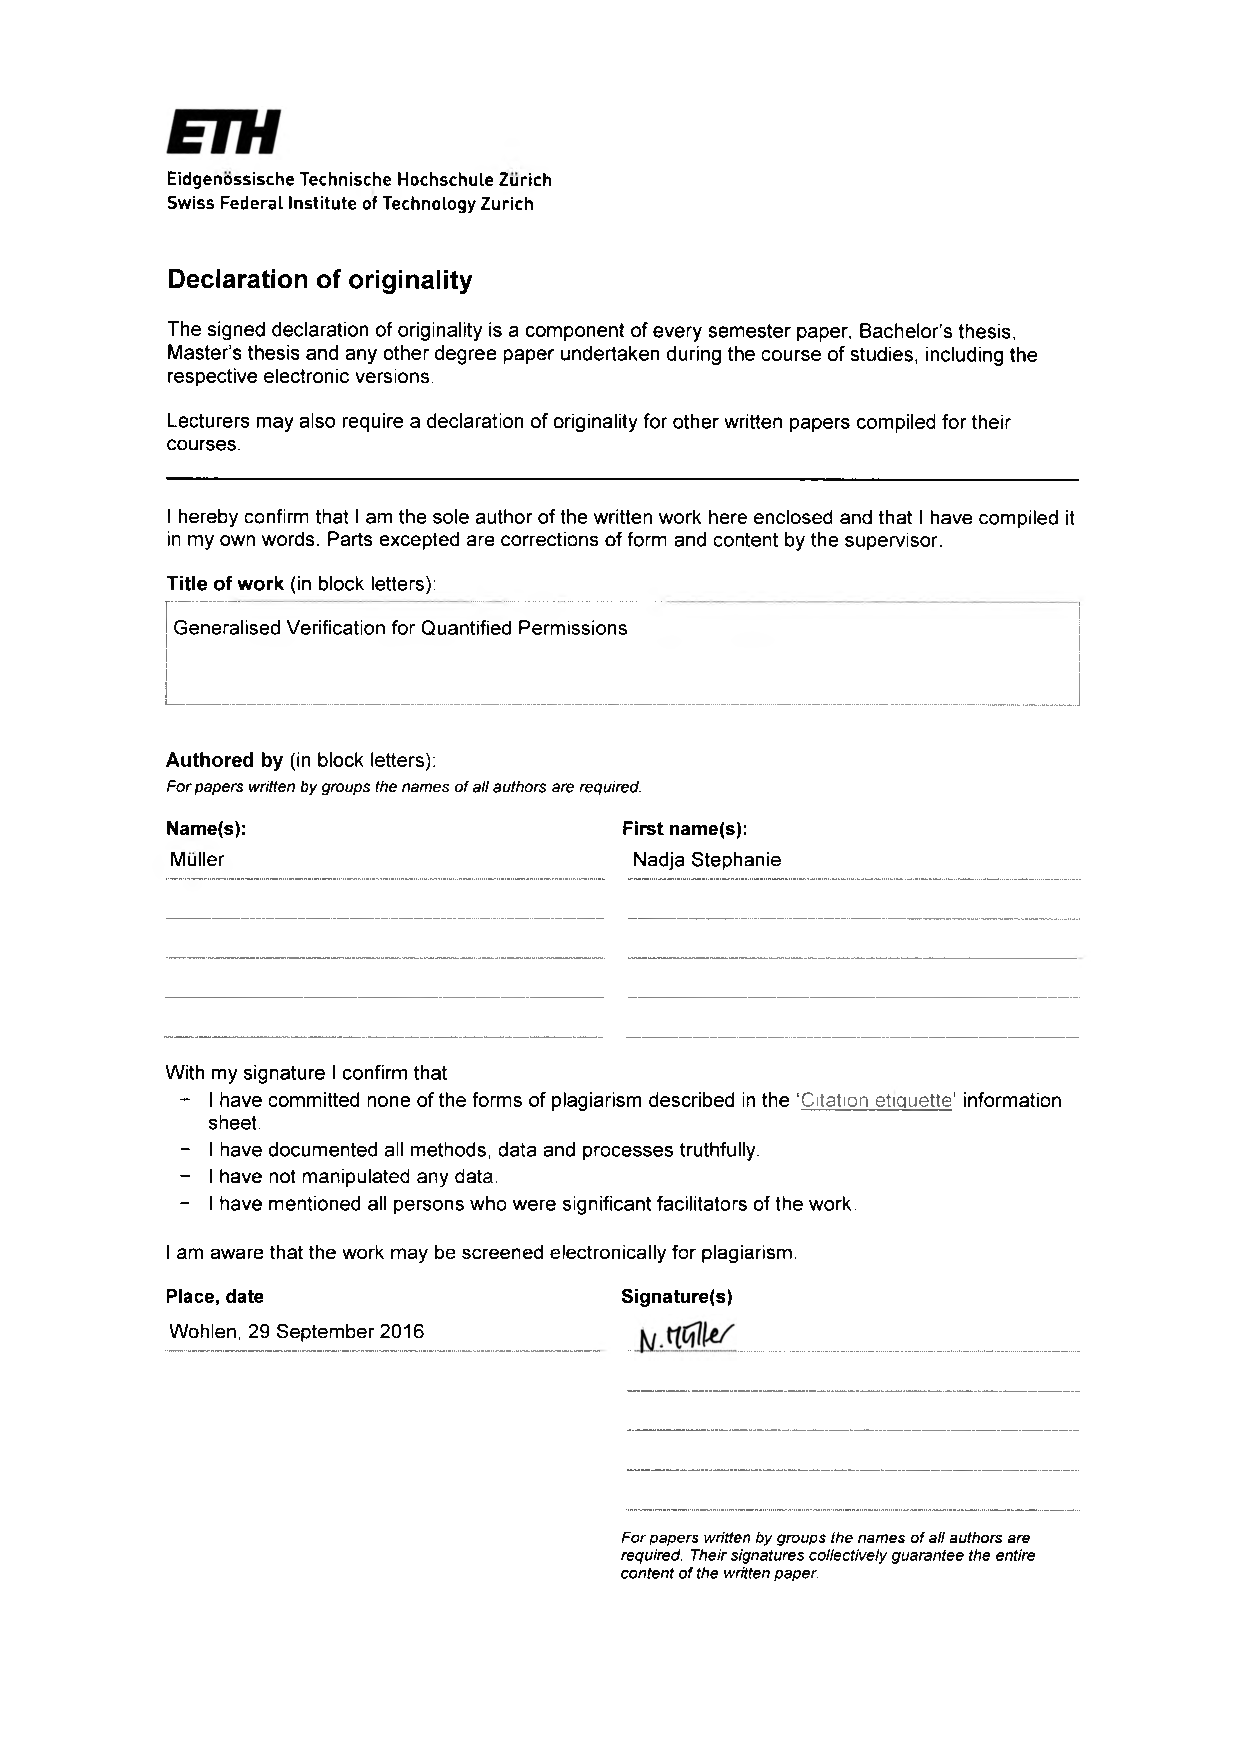
\includepdf[pages={1}]{declaration.pdf}
\end{document}